% Options for packages loaded elsewhere
\PassOptionsToPackage{unicode}{hyperref}
\PassOptionsToPackage{hyphens}{url}
\PassOptionsToPackage{dvipsnames,svgnames,x11names}{xcolor}
%
\documentclass[
  letterpaper,
  DIV=11,
  numbers=noendperiod,
  titlepage=false]{scrreprt}

\usepackage{amsmath,amssymb}
\usepackage{iftex}
\ifPDFTeX
  \usepackage[T1]{fontenc}
  \usepackage[utf8]{inputenc}
  \usepackage{textcomp} % provide euro and other symbols
\else % if luatex or xetex
  \usepackage{unicode-math}
  \defaultfontfeatures{Scale=MatchLowercase}
  \defaultfontfeatures[\rmfamily]{Ligatures=TeX,Scale=1}
\fi
\usepackage{lmodern}
\ifPDFTeX\else  
    % xetex/luatex font selection
\fi
% Use upquote if available, for straight quotes in verbatim environments
\IfFileExists{upquote.sty}{\usepackage{upquote}}{}
\IfFileExists{microtype.sty}{% use microtype if available
  \usepackage[]{microtype}
  \UseMicrotypeSet[protrusion]{basicmath} % disable protrusion for tt fonts
}{}
\makeatletter
\@ifundefined{KOMAClassName}{% if non-KOMA class
  \IfFileExists{parskip.sty}{%
    \usepackage{parskip}
  }{% else
    \setlength{\parindent}{0pt}
    \setlength{\parskip}{6pt plus 2pt minus 1pt}}
}{% if KOMA class
  \KOMAoptions{parskip=half}}
\makeatother
\usepackage{xcolor}
\usepackage[top=30mm,left=20mm,heightrounded]{geometry}
\setlength{\emergencystretch}{3em} % prevent overfull lines
\setcounter{secnumdepth}{5}
% Make \paragraph and \subparagraph free-standing
\ifx\paragraph\undefined\else
  \let\oldparagraph\paragraph
  \renewcommand{\paragraph}[1]{\oldparagraph{#1}\mbox{}}
\fi
\ifx\subparagraph\undefined\else
  \let\oldsubparagraph\subparagraph
  \renewcommand{\subparagraph}[1]{\oldsubparagraph{#1}\mbox{}}
\fi


\providecommand{\tightlist}{%
  \setlength{\itemsep}{0pt}\setlength{\parskip}{0pt}}\usepackage{longtable,booktabs,array}
\usepackage{calc} % for calculating minipage widths
% Correct order of tables after \paragraph or \subparagraph
\usepackage{etoolbox}
\makeatletter
\patchcmd\longtable{\par}{\if@noskipsec\mbox{}\fi\par}{}{}
\makeatother
% Allow footnotes in longtable head/foot
\IfFileExists{footnotehyper.sty}{\usepackage{footnotehyper}}{\usepackage{footnote}}
\makesavenoteenv{longtable}
\usepackage{graphicx}
\makeatletter
\def\maxwidth{\ifdim\Gin@nat@width>\linewidth\linewidth\else\Gin@nat@width\fi}
\def\maxheight{\ifdim\Gin@nat@height>\textheight\textheight\else\Gin@nat@height\fi}
\makeatother
% Scale images if necessary, so that they will not overflow the page
% margins by default, and it is still possible to overwrite the defaults
% using explicit options in \includegraphics[width, height, ...]{}
\setkeys{Gin}{width=\maxwidth,height=\maxheight,keepaspectratio}
% Set default figure placement to htbp
\makeatletter
\def\fps@figure{htbp}
\makeatother

% load packages
\usepackage{geometry}
\usepackage{xcolor}
\usepackage{eso-pic}
\usepackage{fancyhdr}
\usepackage{sectsty}
\usepackage{fontspec}
\usepackage{titlesec}
\usepackage{tabularx}
\usepackage{etoolbox}
\usepackage{graphicx}

%% Set page size with a wider left margin
\geometry{a4paper, total={170mm,257mm}, left=54mm, top=35mm, bottom=25mm, right=15mm}

%% Define colours
\definecolor{light}{HTML}{3E6682}
\definecolor{highlight}{HTML}{000000}
\definecolor{dark}{HTML}{103A60}

%% Add border on the left-hand side
%%\AddToShipoutPicture{% 
%%    \AtPageLowerLeft{% 
%%        \put(\LenToUnit{\dimexpr\paperwidth-21cm},0){% 
%%            \color{light}\rule{3cm}{\LenToUnit\paperheight}%
%%          }%
%%     }%
%%     % logo
%%    \AtPageLowerLeft{% start the bar at the bottom right of the page
%%        \put(.80cm,27.2cm){% move it to the top right
%%            \color{light}
\includegraphics[width=1.5cm]{_extensions/cday/RtpPDF/wftdm-logo.png}
%%          }%
%%     }%
%%}

% Add watermark
\usepackage{eso-pic}
\usepackage{graphicx}
\usepackage{transparent}

\AddToShipoutPictureBG{%
    \begin{tikzpicture}[remember picture,overlay]
        \node[opacity=0.25,inner sep=0pt,anchor=north west] at (current page.north west) {
\includegraphics[height=\paperheight,width=\paperheight,keepaspectratio]{_extensions/cday/RtpPDF/watermark6.png}};
    \end{tikzpicture}%
}

% Make watermark full color on title page
\AddToShipoutPictureBG*{%
    \ifnum\value{page}=1
        \begin{tikzpicture}[remember picture,overlay]
            \node[inner sep=0pt,anchor=north west] at (current page.north west) {
\includegraphics[height=\paperheight,width=\paperwidth,keepaspectratio]{_extensions/cday/RtpPDF/watermark6.png}};
        \end{tikzpicture}%
    \fi
}

% Add page numbers and sponsor png to bottom of pages
\fancypagestyle{mystyle}{
  \fancyhf{}
  \renewcommand\headrulewidth{0pt}
  \fancyfoot[C]{\ifnum\value{page}>1\hspace{-3cm}\textcolor{dark}{\textbf{\thepage}}\fi}
  \fancyfoot[L]{\ifnum\value{page}>1\textcolor{dark}{\textbf{What's New? - Version 9.0.0}}\fi}
  \fancyfootoffset{3.5cm}
  \AddToShipoutPictureBG{%
    \AtPageLowerLeft{
      \ifnum\value{page}>1
        \put(-2.50cm,.9cm){
          \hspace{\dimexpr\paperwidth-2cm}\hspace*{-2cm}\vspace*{2cm}
\includegraphics[width=5cm, height=5cm]{_extensions/cday/RtpPDF/sponsors2.png}
        }
      \fi  
      \put(\LenToUnit{1.2cm}, \LenToUnit{2cm}){%
        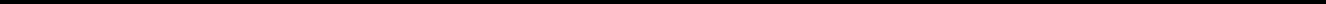
\includegraphics[width=19cm, height=5cm]{_extensions/cday/RtpPDF/footer-line.png}%
      }
    }%
  }
}
\setlength{\footskip}{35pt}


\usepackage{titlesec}
\titleformat{\subsubsection}
  {\normalfont\bfseries}{\thesubsubsection.}{1em}{}
\setcounter{secnumdepth}{4}

%% Style the chapter/section fonts
\chapterfont{\color{dark}\fontsize{28}{15}\selectfont}
\sectionfont{\color{light}\fontsize{20}{15}\selectfont}
\subsectionfont{\color{light}\fontsize{16}{15}\selectfont}
\subsubsectionfont{\color{light}\fontsize{13}{15}\selectfont}

% Redefine \@makechapterhead to format chapter titles
\makeatletter
\renewcommand{\@makechapterhead}[1]{%
  \vspace*{-30pt}% Adjust the vertical spacing before the chapter title
  {\parindent \z@ \raggedright \normalfont
    \ifnum \c@secnumdepth >\m@ne
      \if@mainmatter
        \color{dark}\sffamily\Huge\bfseries \thechapter\hspace{0.5em}% Add two spaces after chapter number
      \fi
    \fi
    \interlinepenalty\@M
    \sffamily\Huge \bfseries #1\par % Chapter title formatting
    \nobreak
    \vskip 40\p@ % Adjust the vertical spacing after the chapter title
  }}
\makeatother

\makeatletter
\renewcommand{\maketitle}{\bgroup\setlength{\parindent}{0pt}
\begin{flushleft}
  \vspace*{\baselineskip}
  \vspace*{\baselineskip}
  {\sffamily\Huge\textbf{\MakeUppercase{\@title}}} \vspace{0.3cm} \newline \newline
  {\LARGE {\@subtitle}}
  \@author \newline \newline
  \@date % Display the date
\end{flushleft}\egroup
}
\makeatother

%% Use custom fonts
\setsansfont{AzoSans}[
    Path=_extensions/cday/RtpPDF/AzoSans/,
    Scale=0.9,
    Extension = .ttf,
    UprightFont=*-Regular,
    BoldFont=*-Bold,
    ItalicFont=*-Italic,
]

\setmainfont{AzoSans}[
    Path=_extensions/cday/RtpPDF/AzoSans/,
    Scale=0.9,
    Extension = .ttf,
    UprightFont=*-Regular,
    BoldFont=*-Bold,
    ItalicFont=*-Italic,
]

\usepackage{enumitem}
\usepackage{graphicx}

\renewcommand{\labelitemi}{
\includegraphics[width=0.5cm]{_extensions/cday/RtpPDF/rtp_bullet2.png}}
\renewcommand{\labelitemii}{
\includegraphics[width=0.5cm]{_extensions/cday/RtpPDF/rtp_bullet2.png}}
\renewcommand{\labelitemiii}{
\includegraphics[width=0.5cm]{_extensions/cday/RtpPDF/rtp_bullet2.png}}
\renewcommand{\labelitemiv}{
\includegraphics[width=0.5cm]{_extensions/cday/RtpPDF/rtp_bullet2.png}}

\KOMAoption{captions}{tableheading}
\makeatletter
\makeatother
\makeatletter
\@ifpackageloaded{bookmark}{}{\usepackage{bookmark}}
\makeatother
\makeatletter
\@ifpackageloaded{caption}{}{\usepackage{caption}}
\AtBeginDocument{%
\ifdefined\contentsname
  \renewcommand*\contentsname{Table of contents}
\else
  \newcommand\contentsname{Table of contents}
\fi
\ifdefined\listfigurename
  \renewcommand*\listfigurename{List of Figures}
\else
  \newcommand\listfigurename{List of Figures}
\fi
\ifdefined\listtablename
  \renewcommand*\listtablename{List of Tables}
\else
  \newcommand\listtablename{List of Tables}
\fi
\ifdefined\figurename
  \renewcommand*\figurename{Figure}
\else
  \newcommand\figurename{Figure}
\fi
\ifdefined\tablename
  \renewcommand*\tablename{Table}
\else
  \newcommand\tablename{Table}
\fi
}
\@ifpackageloaded{float}{}{\usepackage{float}}
\floatstyle{ruled}
\@ifundefined{c@chapter}{\newfloat{codelisting}{h}{lop}}{\newfloat{codelisting}{h}{lop}[chapter]}
\floatname{codelisting}{Listing}
\newcommand*\listoflistings{\listof{codelisting}{List of Listings}}
\makeatother
\makeatletter
\@ifpackageloaded{caption}{}{\usepackage{caption}}
\@ifpackageloaded{subcaption}{}{\usepackage{subcaption}}
\makeatother
\makeatletter
\@ifpackageloaded{tcolorbox}{}{\usepackage[skins,breakable]{tcolorbox}}
\makeatother
\makeatletter
\@ifundefined{shadecolor}{\definecolor{shadecolor}{rgb}{.97, .97, .97}}
\makeatother
\makeatletter
\@ifundefined{codebgcolor}{\definecolor{codebgcolor}{named}{light}}
\makeatother
\makeatletter
\makeatother
\ifLuaTeX
  \usepackage{selnolig}  % disable illegal ligatures
\fi
\IfFileExists{bookmark.sty}{\usepackage{bookmark}}{\usepackage{hyperref}}
\IfFileExists{xurl.sty}{\usepackage{xurl}}{} % add URL line breaks if available
\urlstyle{same} % disable monospaced font for URLs
\hypersetup{
  pdftitle={What's New? - Version 9.0.0},
  pdfauthor={WFRC / MAG},
  colorlinks=true,
  linkcolor={highlight},
  filecolor={Maroon},
  citecolor={Blue},
  urlcolor={highlight},
  pdfcreator={LaTeX via pandoc}}

\title{What's New? - Version 9.0.0}
\author{WFRC / MAG}
\date{August 1, 2023}

\begin{document}
\maketitle
\pagestyle{mystyle}

\ifdefined\Shaded\renewenvironment{Shaded}{\begin{tcolorbox}[frame hidden, breakable, boxrule=0pt, sharp corners, borderline west={3pt}{0pt}{shadecolor}, colback={codebgcolor}, enhanced]}{\end{tcolorbox}}\fi

\renewcommand*\contentsname{Table of contents}
{
\hypersetup{linkcolor=}
\setcounter{tocdepth}{2}
\tableofcontents
}
\listoffigures
\listoftables
\bookmarksetup{startatroot}

\hypertarget{documentation}{%
\chapter{Documentation}\label{documentation}}

Documentation of the Wasatch Front Travel Demand Model (WF TDM) has been
separated into three documents:

\begin{itemize}
\tightlist
\item
  What's New Report -- describes the changes made to the WF TDM since
  the last model release
\item
  Validation Report -- provides the base year validation of the current
  version of the WF TDM, as well as a reasonableness check of the model
  as a forecasting tool
\item
  Model Process Report -- provides an overview of the model, a summary
  of the model's input data sets, and an outline of the model's primary
  steps and logic
\end{itemize}

These reports will be available as PDF documents in the ``\_Notes''
folder in the WF TDM's root directory. However, it is expected that the
primary means of accessing the model's documentation will be online at
the following links:

\begin{itemize}
\tightlist
\item
  \href{https://wfrc.org/wftdm-docs/v9x/v900/whats-new/1-genparams.html}{What's
  New}
\item
  \href{https://wfrc.org/wftdm-docs/v9x/v900/validation/1-hhdisag-autoown.html}{Validation
  Report}
\item
  Model Process Report (in progress)
\item
  Previous Versions (in progress)
\end{itemize}

\bookmarksetup{startatroot}

\hypertarget{general-parameters}{%
\chapter{General Parameters}\label{general-parameters}}

Changes made to the \texttt{0\_GeneralParameters.block} file are
discussed in this section.

\hypertarget{zone-parameters}{%
\section{Zone Parameters}\label{zone-parameters}}

The TAZ and highway node schema was changed as a result of the version 9
TAZ splits. The following parameters were updated to reflect these
changes.

\hypertarget{taz}{%
\subsection{TAZ}\label{taz}}

\hypertarget{tbl-taz-ranges}{}
\begin{longtable}[]{@{}
  >{\raggedright\arraybackslash}p{(\columnwidth - 6\tabcolsep) * \real{0.2000}}
  >{\raggedright\arraybackslash}p{(\columnwidth - 6\tabcolsep) * \real{0.2000}}
  >{\raggedright\arraybackslash}p{(\columnwidth - 6\tabcolsep) * \real{0.3000}}
  >{\raggedright\arraybackslash}p{(\columnwidth - 6\tabcolsep) * \real{0.3000}}@{}}
\caption{\label{tbl-taz-ranges}Renumbered TAZ Ranges}\tabularnewline
\toprule\noalign{}
\begin{minipage}[b]{\linewidth}\raggedright
Parameter
\end{minipage} & \begin{minipage}[b]{\linewidth}\raggedright
v9 Value
\end{minipage} & \begin{minipage}[b]{\linewidth}\raggedright
v8 Value
\end{minipage} & \begin{minipage}[b]{\linewidth}\raggedright
Notes
\end{minipage} \\
\midrule\noalign{}
\endfirsthead
\toprule\noalign{}
\begin{minipage}[b]{\linewidth}\raggedright
Parameter
\end{minipage} & \begin{minipage}[b]{\linewidth}\raggedright
v9 Value
\end{minipage} & \begin{minipage}[b]{\linewidth}\raggedright
v8 Value
\end{minipage} & \begin{minipage}[b]{\linewidth}\raggedright
Notes
\end{minipage} \\
\midrule\noalign{}
\endhead
\bottomrule\noalign{}
\endlastfoot
UsedZones & 3629 & 2881 & Highest TAZ number used by model \\
BoxElderRange & 1-153 & 1-140 & Box Elder County Range \\
WeberRange & 154-581 & 141-423 & Weber County Range \\
DavisRange & 582-905 & 424-654 & Davis County Range \\
SLRange & 906-2216 & 655-1788 & Salt Lake County Range \\
UtahRange & 2217-3546 & 1789-2881 & Utah County Range \\
Dummyzones & 3547-3600 & 2882-3400 & Placeholder for future TAZ
splits \\
Externalzones & 3601-3629 & 136-140, 421-423, 1782-1788, 2874-2881 &
External zones \\
NorthBC & 3604-3606 & 138, 139, 140 & North Brigham City external
zones \\
\end{longtable}

The following TAZ parameters ranges were removed from the general
parameters file as they were not being used in the WF TDM:

\begin{itemize}
\tightlist
\item
  RegionRange
\item
  WFRCRange
\item
  MAGRange
\end{itemize}

\hypertarget{highway-nodes}{%
\subsection{Highway Nodes}\label{highway-nodes}}

\hypertarget{tbl-highway-renumber}{}
\begin{longtable}[]{@{}llll@{}}
\caption{\label{tbl-highway-renumber}Renumbered Highway
Nodes}\label{T_b1fb5}\tabularnewline
\toprule\noalign{}
Parameter & v9 Value & v8 Value & Notes \\
\midrule\noalign{}
\endfirsthead
\toprule\noalign{}
Parameter & v9 Value & v8 Value & Notes \\
\midrule\noalign{}
\endhead
\bottomrule\noalign{}
\endlastfoot
HwyNodes & 10000-99999 & 3401-999999 & Highway and transit node range \\
\end{longtable}

\hypertarget{college-zones}{%
\subsection{College Zones}\label{college-zones}}

Where noted, several colleges were effectively discontinued, meaning
references to these schools are still in the code base, but enrollment
was set to zero.

\hypertarget{tbl-college-renumber}{}
\begin{longtable}[]{@{}
  >{\raggedright\arraybackslash}p{(\columnwidth - 8\tabcolsep) * \real{0.2000}}
  >{\raggedright\arraybackslash}p{(\columnwidth - 8\tabcolsep) * \real{0.2000}}
  >{\raggedright\arraybackslash}p{(\columnwidth - 8\tabcolsep) * \real{0.1100}}
  >{\raggedright\arraybackslash}p{(\columnwidth - 8\tabcolsep) * \real{0.1100}}
  >{\raggedright\arraybackslash}p{(\columnwidth - 8\tabcolsep) * \real{0.3800}}@{}}
\caption{\label{tbl-college-renumber}Renumbered College
Zones}\tabularnewline
\toprule\noalign{}
\begin{minipage}[b]{\linewidth}\raggedright
Area
\end{minipage} & \begin{minipage}[b]{\linewidth}\raggedright
Parameter
\end{minipage} & \begin{minipage}[b]{\linewidth}\raggedright
v9 Value
\end{minipage} & \begin{minipage}[b]{\linewidth}\raggedright
v8 Value
\end{minipage} & \begin{minipage}[b]{\linewidth}\raggedright
Notes
\end{minipage} \\
\midrule\noalign{}
\endfirsthead
\toprule\noalign{}
\begin{minipage}[b]{\linewidth}\raggedright
Area
\end{minipage} & \begin{minipage}[b]{\linewidth}\raggedright
Parameter
\end{minipage} & \begin{minipage}[b]{\linewidth}\raggedright
v9 Value
\end{minipage} & \begin{minipage}[b]{\linewidth}\raggedright
v8 Value
\end{minipage} & \begin{minipage}[b]{\linewidth}\raggedright
Notes
\end{minipage} \\
\midrule\noalign{}
\endhead
\bottomrule\noalign{}
\endlastfoot
WFRC Colleges & Ensign (was LDSBC) & 1029 & 950 & Ensign College \\
& Westmin & 1263 & 1150 & Westminster College \\
& UOFU\_Main & 1051 & 1075 & University of Utah - Main \\
& UOFU\_Med & 1007 & 1076 & University of Utah - Medical (removed) \\
& WSU\_Main (was WSU\_OGDEN) & 437 & 383 & Weber State University -
Main \\
& WSU\_Davis & 693 & 525 & Weber State University - Davis \\
& WSU\_West & 521 & 290 & Weber State University - West (removed) \\
& SLCC\_Main (was SLCC\_TL) & 1580 & 897 & Salt Lake Community College -
Main \\
& SLCC\_SC & 1231 & 1126 & Salt Lake Community College - South City \\
& SLCC\_JD & 1776 & 1493 & Salt Lake Community College - Jordan \\
& SLCC\_Mead & & 1206 & Salt Lake Community College - Meadbrook
(removed) \\
& SLCC\_ML & 1886 & 1516 & Salt Lake Community College - Miller \\
& SLCC\_LB & 1085 & 989 & Salt Lake Community College - Library
(removed) \\
& SLCC\_HL & 1525 & 1294 & Salt Lake Community College - Highland
(removed) \\
& SLCC\_Airp & 979 & 746 & Salt Lake Community College - Airport
(removed) \\
& SLCC\_West & 959 & 745 & Salt Lake Community College - Westpointe
(removed) \\
& SLCC\_HM & 2031 & 1607 & Salt Lake Community College - Herriman
(removed) \\
MAG Colleges & BYU & 2939 & 2384 & Brigham Young University - Main \\
& UVU\_Main & 2848 & 2326 & Utah Valley University - Main \\
& UVU\_Geneva & 2882 & 2280 & Utah Valley University - Geneva
(removed) \\
& UVU\_Lehi (was UVU\_THANKP) & 2606 & 2099 & Utah Valley University -
Lehi \\
& UVU\_Vine & 2809 & 2259 & Utah Valley University - Vineyard \\
& UVU\_Payson & 3336 & 2690 & Utah Valley University - Payson \\
\end{longtable}

\hypertarget{tbl-college-renumber-2}{}
\begin{longtable}[]{@{}
  >{\raggedright\arraybackslash}p{(\columnwidth - 4\tabcolsep) * \real{0.1500}}
  >{\raggedright\arraybackslash}p{(\columnwidth - 4\tabcolsep) * \real{0.4000}}
  >{\raggedright\arraybackslash}p{(\columnwidth - 4\tabcolsep) * \real{0.4500}}@{}}
\caption{\label{tbl-college-renumber-2}Renumbered College Zones
(continued)}\tabularnewline
\toprule\noalign{}
\begin{minipage}[b]{\linewidth}\raggedright
Parameter
\end{minipage} & \begin{minipage}[b]{\linewidth}\raggedright
v9 Value
\end{minipage} & \begin{minipage}[b]{\linewidth}\raggedright
v8 Value
\end{minipage} \\
\midrule\noalign{}
\endfirsthead
\toprule\noalign{}
\begin{minipage}[b]{\linewidth}\raggedright
Parameter
\end{minipage} & \begin{minipage}[b]{\linewidth}\raggedright
v9 Value
\end{minipage} & \begin{minipage}[b]{\linewidth}\raggedright
v8 Value
\end{minipage} \\
\midrule\noalign{}
\endhead
\bottomrule\noalign{}
\endlastfoot
colleges & 437, 521, 693, 959, 979, 1007, 1029, 1051, 1085, 1231, 1263,
1491, 1525, 1580, 1776, 1886, 2031, 2606, 2809, 2848, 2882, 2939, 3336 &
290, 383, 525, 897, 950, 989, 1075, 1076, 1126, 1150, 1294, 1493, 1516,
1607, 2099, 2259, 2280, 2326, 2384, 2690 \\
\end{longtable}

\hypertarget{zones-with-off-line-trip-tables}{%
\subsection{Zones with Off-line Trip
Tables}\label{zones-with-off-line-trip-tables}}

\hypertarget{tbl-offline-renumber}{}
\begin{longtable}[]{@{}lll@{}}
\caption{\label{tbl-offline-renumber}Renumbered Off-line Trip Table
Zones}\label{T_b41aa}\tabularnewline
\toprule\noalign{}
Parameter & v9 Value & v8 Value \\
\midrule\noalign{}
\endfirsthead
\toprule\noalign{}
Parameter & v9 Value & v8 Value \\
\midrule\noalign{}
\endhead
\bottomrule\noalign{}
\endlastfoot
Lagoon & 781 & 562 \\
Airport & 965 & 742 \\
\end{longtable}

\hypertarget{special-generator-zones}{%
\subsection{Special Generator Zones}\label{special-generator-zones}}

\hypertarget{tbl-specgen-renumber}{}
\begin{longtable}[]{@{}lll@{}}
\caption{\label{tbl-specgen-renumber}Renumbered Special Generator
Zones}\label{T_dc81e}\tabularnewline
\toprule\noalign{}
Parameter & v9 Value & v8 Value \\
\midrule\noalign{}
\endfirsthead
\toprule\noalign{}
Parameter & v9 Value & v8 Value \\
\midrule\noalign{}
\endhead
\bottomrule\noalign{}
\endlastfoot
TempleSquare & 1035 & 966 \\
SLC\_Library & 1147 & 1015 \\
\end{longtable}

\hypertarget{exogenous-trip-table-parameters}{%
\section{Exogenous Trip Table
Parameters}\label{exogenous-trip-table-parameters}}

Income break points for the airport exogenous trip table generation were
updated to reflect 2019 base year income.

\newpage

\hypertarget{tbl-exogen-income}{}
\begin{longtable}[]{@{}llll@{}}
\caption{\label{tbl-exogen-income}Income Break Points for Airport
Exogenous Trip Table Generation}\label{T_daa27}\tabularnewline
\toprule\noalign{}
Parameter & v9 Value & v8 Value & Notes \\
\midrule\noalign{}
\endfirsthead
\toprule\noalign{}
Parameter & v9 Value & v8 Value & Notes \\
\midrule\noalign{}
\endhead
\bottomrule\noalign{}
\endlastfoot
Income\_Lo & \$45,000 & \$35,000 & breakpoint between Inc1 \& Inc2 \\
Income\_Md & \$75,000 & \$70,000 & breakpoint between Inc2 \& Inc3 \\
Income\_Hi & \$125,000 & \$100,000 & breakpoint between Inc3 \& Inc4 \\
\end{longtable}

\hypertarget{household-disaggregation-parameters}{%
\section{Household Disaggregation
Parameters}\label{household-disaggregation-parameters}}

The regional median income was updated using 2019 5-year ACS data and
kept in 2019 dollars to reflect 2019 base year. Note, the version 8
value was estimated from 2015 ACS data and deflated to 2010 dollars.

\hypertarget{tbl-hh-disagg}{}
\begin{longtable}[]{@{}lll@{}}
\caption{\label{tbl-hh-disagg}Household Disaggregation Parameter Income
Update}\label{T_527df}\tabularnewline
\toprule\noalign{}
Parameter & v9 Value & v8 Value \\
\midrule\noalign{}
\endfirsthead
\toprule\noalign{}
Parameter & v9 Value & v8 Value \\
\midrule\noalign{}
\endhead
\bottomrule\noalign{}
\endlastfoot
Reg\_Median\_Inc & \$74,946 & \$58,793 \\
\end{longtable}

\hypertarget{distribution-mode-choice-and-assignment-parameters}{%
\section{Distribution, Mode Choice, and Assignment
Parameters}\label{distribution-mode-choice-and-assignment-parameters}}

\hypertarget{k-factors}{%
\subsection{K-Factors}\label{k-factors}}

K-factor variables were expanded by trip purpose to allow for more
flexibility in calibrating the distribution model. However, no K-factors
were needed for calibration. All K-factors were reset to 1.

\hypertarget{tbl-kfactors}{}
\begin{longtable}[]{@{}
  >{\raggedright\arraybackslash}p{(\columnwidth - 8\tabcolsep) * \real{0.3700}}
  >{\raggedright\arraybackslash}p{(\columnwidth - 8\tabcolsep) * \real{0.2300}}
  >{\raggedright\arraybackslash}p{(\columnwidth - 8\tabcolsep) * \real{0.1100}}
  >{\raggedright\arraybackslash}p{(\columnwidth - 8\tabcolsep) * \real{0.1800}}
  >{\raggedright\arraybackslash}p{(\columnwidth - 8\tabcolsep) * \real{0.1100}}@{}}
\caption{\label{tbl-kfactors}Reset K-Factors}\tabularnewline
\toprule\noalign{}
\begin{minipage}[b]{\linewidth}\raggedright
Area
\end{minipage} & \begin{minipage}[b]{\linewidth}\raggedright
v9 Parameter
\end{minipage} & \begin{minipage}[b]{\linewidth}\raggedright
v9 Value
\end{minipage} & \begin{minipage}[b]{\linewidth}\raggedright
v8 Parameter
\end{minipage} & \begin{minipage}[b]{\linewidth}\raggedright
v8 Value
\end{minipage} \\
\midrule\noalign{}
\endfirsthead
\toprule\noalign{}
\begin{minipage}[b]{\linewidth}\raggedright
Area
\end{minipage} & \begin{minipage}[b]{\linewidth}\raggedright
v9 Parameter
\end{minipage} & \begin{minipage}[b]{\linewidth}\raggedright
v9 Value
\end{minipage} & \begin{minipage}[b]{\linewidth}\raggedright
v8 Parameter
\end{minipage} & \begin{minipage}[b]{\linewidth}\raggedright
v8 Value
\end{minipage} \\
\midrule\noalign{}
\endhead
\bottomrule\noalign{}
\endlastfoot
between Salt Lake and Utah counties & SL\_UT\_KFAC\_Wrk & 1 &
SL\_UT\_KFAC & 0.85 \\
& SL\_UT\_KFAC\_Oth & 1 & & \\
& SL\_UT\_KFAC\_Trk & 1 & & \\
& SL\_UT\_KFAC\_Ext & 1 & & \\
between Salt Lake and Davis counties & SL\_DA\_KFAC\_Wrk & 1 &
SL\_DA\_KFAC & 0.95 \\
& SL\_DA\_KFAC\_Oth & 1 & & \\
& SL\_DA\_KFAC\_Trk & 1 & & \\
& SL\_DA\_KFAC\_Ext & 1 & & \\
between Box Elder and Weber counties & WE\_BE\_KFAC\_Wrk & 1 &
WE\_BE\_KFAC & 1.00 \\
& WE\_BE\_KFAC\_Oth & 1 & & \\
& WE\_BE\_KFAC\_Trk & 1 & & \\
& WE\_BE\_KFAC\_Ext & 1 & & \\
\end{longtable}

\hypertarget{auto-occupancy}{%
\subsection{Auto Occupancy}\label{auto-occupancy}}

Auto or vehicle occupancy variables were expanded to include additional
trips purposes. New auto-occupancy rates were calculated based on the
reprocessed 2012 Household Travel Survey. Values represent average
persons per vehicle for just the Wasatch Front model space. External
auto-occupancy rates represent the average of internal-external and
external-internal trips.

\hypertarget{tbl-auto-occ1}{}
\begin{longtable}[]{@{}
  >{\raggedright\arraybackslash}p{(\columnwidth - 8\tabcolsep) * \real{0.2000}}
  >{\raggedright\arraybackslash}p{(\columnwidth - 8\tabcolsep) * \real{0.0800}}
  >{\raggedright\arraybackslash}p{(\columnwidth - 8\tabcolsep) * \real{0.3500}}
  >{\raggedright\arraybackslash}p{(\columnwidth - 8\tabcolsep) * \real{0.0800}}
  >{\raggedright\arraybackslash}p{(\columnwidth - 8\tabcolsep) * \real{0.2900}}@{}}
\caption{\label{tbl-auto-occ1}Vehicle Occupancy Rates}\tabularnewline
\toprule\noalign{}
\begin{minipage}[b]{\linewidth}\raggedright
v9 Parameter
\end{minipage} & \begin{minipage}[b]{\linewidth}\raggedright
v9 Value
\end{minipage} & \begin{minipage}[b]{\linewidth}\raggedright
v8 Parameter
\end{minipage} & \begin{minipage}[b]{\linewidth}\raggedright
v8 Value
\end{minipage} & \begin{minipage}[b]{\linewidth}\raggedright
Notes
\end{minipage} \\
\midrule\noalign{}
\endfirsthead
\toprule\noalign{}
\begin{minipage}[b]{\linewidth}\raggedright
v9 Parameter
\end{minipage} & \begin{minipage}[b]{\linewidth}\raggedright
v9 Value
\end{minipage} & \begin{minipage}[b]{\linewidth}\raggedright
v8 Parameter
\end{minipage} & \begin{minipage}[b]{\linewidth}\raggedright
v8 Value
\end{minipage} & \begin{minipage}[b]{\linewidth}\raggedright
Notes
\end{minipage} \\
\midrule\noalign{}
\endhead
\bottomrule\noalign{}
\endlastfoot
VehOcc\_HBW & 1.1 & VEH\_OCCUPANCY\_HBW & 1.1 & Home-Based Work \\
VehOcc\_HBShp & 1.63 & VEH\_OCCUPANCY\_HBSHP & 1.58 & Home-Based
Shopping \\
VehOcc\_HBOth & 1.68 & VEH\_OCCUPANCY\_HBOTH & 1.66 & Home-Based
Other \\
VehOcc\_HBSch & 1.76 & VEH\_OCCUPANCY\_HBSCH & 2.14 & Home-Based
School \\
VehOcc\_HBC & 1.12 & VEH\_OCCUPANCY\_HBC & 1.26 & Home-Based College \\
VehOcc\_NHBW & 1.21 & VEH\_OCCUPANCY\_NHBW & 1.2 & Non-Home-Based
Work \\
VehOcc\_NHBNW & 1.76 & VEH\_OCCUPANCY\_NHBNW & 1.7 & Non-Home-Based
Non-Work \\
VehOcc\_Rec & 1.68 & (Uses HBO) & 1.64 & Recreation \\
VehOcc\_HBO & 1.67 & VEH\_OCCUPANCY\_HBO & 1.64 & Home-Based Other
(HBShp+HBOth) \\
VehOcc\_NHB & 1.54 & VEH\_OCCUPANCY\_NHB & 1.48 & Non-Home-Based
(NHBW+NHBNW) \\
VehOcc\_ExtWrk & 1.16 & (Uses HBW) & 1.1 & External Work \\
VehOcc\_ExtHBO & 1.82 & (Uses HBO) & 1.64 & External Home-Based Other \\
VehOcc\_ExtNHB & 1.73 & (Uses NHB) & 1.48 & Non-Home-Based \\
VehOcc\_ExtRec & 1.73 & (Uses HBO) & 1.64 & External Recreation \\
\end{longtable}

\hypertarget{tbl-auto-occ2}{}
\begin{longtable}[]{@{}
  >{\raggedright\arraybackslash}p{(\columnwidth - 8\tabcolsep) * \real{0.2400}}
  >{\raggedright\arraybackslash}p{(\columnwidth - 8\tabcolsep) * \real{0.0800}}
  >{\raggedright\arraybackslash}p{(\columnwidth - 8\tabcolsep) * \real{0.2400}}
  >{\raggedright\arraybackslash}p{(\columnwidth - 8\tabcolsep) * \real{0.0800}}
  >{\raggedright\arraybackslash}p{(\columnwidth - 8\tabcolsep) * \real{0.3600}}@{}}
\caption{\label{tbl-auto-occ2}Vehicle Occupancy 3+ Rates}\tabularnewline
\toprule\noalign{}
\begin{minipage}[b]{\linewidth}\raggedright
v9 Parameter
\end{minipage} & \begin{minipage}[b]{\linewidth}\raggedright
v9 Value
\end{minipage} & \begin{minipage}[b]{\linewidth}\raggedright
v8 Parameter
\end{minipage} & \begin{minipage}[b]{\linewidth}\raggedright
v8 Value
\end{minipage} & \begin{minipage}[b]{\linewidth}\raggedright
Notes
\end{minipage} \\
\midrule\noalign{}
\endfirsthead
\toprule\noalign{}
\begin{minipage}[b]{\linewidth}\raggedright
v9 Parameter
\end{minipage} & \begin{minipage}[b]{\linewidth}\raggedright
v9 Value
\end{minipage} & \begin{minipage}[b]{\linewidth}\raggedright
v8 Parameter
\end{minipage} & \begin{minipage}[b]{\linewidth}\raggedright
v8 Value
\end{minipage} & \begin{minipage}[b]{\linewidth}\raggedright
Notes
\end{minipage} \\
\midrule\noalign{}
\endhead
\bottomrule\noalign{}
\endlastfoot
VehOcc\_3p\_HBW & 3.53 & VEH\_OCC\_3P\_HBW & 3.4 & 3+ Person Home-Based
Work \\
VehOcc\_3p\_HBShp & 3.49 & (Uses HBO) & 3.55 & 3+ Person Home-Based
Shopping \\
VehOcc\_3p\_HBOth & 3.73 & (Uses HBO) & 3.55 & 3+ Person Home-Based
Other \\
VehOcc\_3p\_HBSch & 3.88 & (Uses HBO) & 3.55 & 3+ Person Home-Based
School \\
VehOcc\_3p\_HBC & 3.24 & VEH\_OCC\_3P\_HBC & 3.53 & 3+ Person Home-Based
College \\
VehOcc\_3p\_NHBW & 3.71 & (Uses NHB) & 3.51 & 3+ Person Non-Home-Based
Work \\
VehOcc\_3p\_NHBNW & 3.71 & (Uses NHB) & 3.51 & 3+ Person Non-Home-Based
Non-Work \\
VehOcc\_3p\_Rec & 3.73 & (Uses HBO) & 3.55 & 3+ Person Recreation \\
VehOcc\_3p\_HBO & 3.68 & VEH\_OCC\_3P\_HBO & 3.55 & 3+ Person Home-Based
Other (HBShp+HBOth) \\
VehOcc\_3p\_NHB & 3.71 & VEH\_OCC\_3P\_NHB & 3.51 & 3+ Person
Non-Home-Based (NHBW+NHBNW) \\
\end{longtable}

\hypertarget{value-of-time}{%
\subsection{Value of Time}\label{value-of-time}}

Value of time parameters were updated using 2019 5-year ACS data and
previous model assumptions and are in 2019 dollars. Version 8 parameters
were calibrated to 2015 ACS data and deflated to 2010 dollars. Values of
time are in cents/minute.

\hypertarget{tbl-vot1}{}
\begin{longtable}[]{@{}
  >{\raggedright\arraybackslash}p{(\columnwidth - 8\tabcolsep) * \real{0.2400}}
  >{\raggedright\arraybackslash}p{(\columnwidth - 8\tabcolsep) * \real{0.0800}}
  >{\raggedright\arraybackslash}p{(\columnwidth - 8\tabcolsep) * \real{0.2400}}
  >{\raggedright\arraybackslash}p{(\columnwidth - 8\tabcolsep) * \real{0.0800}}
  >{\raggedright\arraybackslash}p{(\columnwidth - 8\tabcolsep) * \real{0.3600}}@{}}
\caption{\label{tbl-vot1}Value of Time Rates}\tabularnewline
\toprule\noalign{}
\begin{minipage}[b]{\linewidth}\raggedright
v9 Parameter
\end{minipage} & \begin{minipage}[b]{\linewidth}\raggedright
v9 Value
\end{minipage} & \begin{minipage}[b]{\linewidth}\raggedright
v8 Parameter
\end{minipage} & \begin{minipage}[b]{\linewidth}\raggedright
v8 Value
\end{minipage} & \begin{minipage}[b]{\linewidth}\raggedright
Notes
\end{minipage} \\
\midrule\noalign{}
\endfirsthead
\toprule\noalign{}
\begin{minipage}[b]{\linewidth}\raggedright
v9 Parameter
\end{minipage} & \begin{minipage}[b]{\linewidth}\raggedright
v9 Value
\end{minipage} & \begin{minipage}[b]{\linewidth}\raggedright
v8 Parameter
\end{minipage} & \begin{minipage}[b]{\linewidth}\raggedright
v8 Value
\end{minipage} & \begin{minipage}[b]{\linewidth}\raggedright
Notes
\end{minipage} \\
\midrule\noalign{}
\endhead
\bottomrule\noalign{}
\endlastfoot
VOT\_Auto\_Wrk & 22 & VOT\_Auto\_Wrk & 18 & work trips (HBW) \\
VOT\_Auto\_Per & 17 & VOT\_Auto\_Per & 14 & non-work trips \\
VOT\_Auto\_Ext & 20 & VOT\_Auto\_Ext & 16 & external \\
VOT\_LT & 37 & VOT\_LT & 30 & light truck \\
VOT\_MD & 50 & VOT\_MD & 40 & medium truck \\
VOT\_HV & 63 & VOT\_HV & 50 & heavy truck \\
VOT\_Toll & 63 & VOT\_Toll & 50 & all vehicles on tollway \\
VOT\_HOT\_DA & 63 & VOT\_HOT\_DA & 50 & drive alone on HOT \\
VOT\_Auto\_Wrk\_Lo & 9 & & & work trips - low income (added) \\
VOT\_Auto\_Wrk\_Hi & 24 & & & work trips - high income (added) \\
VOT\_Auto\_Per\_Lo & 7 & & & non-work trips - loc income (added) \\
VOT\_Auto\_Per\_Hi & 19 & & & non-work trips - high income (added) \\
\end{longtable}

\hypertarget{auto-operating-costs}{%
\subsection{Auto Operating Costs}\label{auto-operating-costs}}

Auto operating costs were updated to reflect 2019 fuel cost, average
fuel economy, and cost of vehicle maintenance and are in 2019 dollars.
Version 8 parameters were calibrated to 2015 data and deflated to 2010
dollars. Costs are in cents/mile.

\hypertarget{tbl-auto-op}{}
\begin{longtable}[]{@{}llll@{}}
\caption{\label{tbl-auto-op}Auto Operating Cost
Rates}\label{T_1af42}\tabularnewline
\toprule\noalign{}
Parameter & v9 Value & v8 Value & Notes \\
\midrule\noalign{}
\endfirsthead
\toprule\noalign{}
Parameter & v9 Value & v8 Value & Notes \\
\midrule\noalign{}
\endhead
\bottomrule\noalign{}
\endlastfoot
AOC\_Auto & 21.7 & 18.3 & auto \\
AOC\_LT & 27.3 & 24.6 & light truck \\
AOC\_MD & 55.5 & 47.8 & medium truck \\
AOC\_HV & 74.3 & 63.7 & heavy truck \\
\end{longtable}

\hypertarget{managed-lane-costs}{%
\subsection{Managed Lane Costs}\label{managed-lane-costs}}

Tolls for tollways (FT=40) were updated to reflect approximately a
\$5.00 toll for work trips and a \$3.00 toll for non-work trips. Tolls
for HOT (FT=38) and reliability lanes were updated to reflect
approximately a \$3.50 toll for work trips and \$2.20 for non-work
trips. Distances of 10.25 miles (length of average work trip) and 6.5
miles (average length of all trips) were used to determine the
work/non-work toll costs in cents per mile. Version 9 tolls are in 2019
dollars. Toll costs for version 8 are in 2010 dollars.

\hypertarget{tbl-managed-lane}{}
\begin{longtable}[]{@{}llll@{}}
\caption{\label{tbl-managed-lane}Managed Lane Cost
Rates}\label{T_8c32b}\tabularnewline
\toprule\noalign{}
Parameter & v9 Value & v8 Value & Notes \\
\midrule\noalign{}
\endfirsthead
\toprule\noalign{}
Parameter & v9 Value & v8 Value & Notes \\
\midrule\noalign{}
\endhead
\bottomrule\noalign{}
\endlastfoot
Cost\_Toll\_Pk & 48 & 24 & Tollways (FT 40) cost - Peak \\
Cost\_Toll\_Ok & 48 & 24 & Tollways (FT 40) cost - Off-peak \\
Cost\_HOT\_Pk & 34 & 10 & HOT (FT 38) cost - Peak \\
Cost\_HOT\_Ok & 17 & 5 & HOT (FT 38) cost - Off-peak \\
Cost\_REL\_Pk & 34 & 10 & Reliability lane cost - Peak \\
Cost\_REL\_Ok & 17 & 5 & Reliability lane cost - Off-peak \\
\end{longtable}

\hypertarget{core-bus-constant-multiplier}{%
\subsection{Core Bus Constant
Multiplier}\label{core-bus-constant-multiplier}}

The parameter used to set the Core Bus constant was renamed and updated.

\hypertarget{tbl-vot2}{}
\begin{longtable}[]{@{}
  >{\raggedright\arraybackslash}p{(\columnwidth - 8\tabcolsep) * \real{0.3000}}
  >{\raggedright\arraybackslash}p{(\columnwidth - 8\tabcolsep) * \real{0.0800}}
  >{\raggedright\arraybackslash}p{(\columnwidth - 8\tabcolsep) * \real{0.3000}}
  >{\raggedright\arraybackslash}p{(\columnwidth - 8\tabcolsep) * \real{0.0800}}
  >{\raggedright\arraybackslash}p{(\columnwidth - 8\tabcolsep) * \real{0.2000}}@{}}
\caption{\label{tbl-vot2}Core Bus Constant Multiplier}\tabularnewline
\toprule\noalign{}
\begin{minipage}[b]{\linewidth}\raggedright
v9 Parameter
\end{minipage} & \begin{minipage}[b]{\linewidth}\raggedright
v9 Value
\end{minipage} & \begin{minipage}[b]{\linewidth}\raggedright
v8 Parameter
\end{minipage} & \begin{minipage}[b]{\linewidth}\raggedright
v8 Value
\end{minipage} & \begin{minipage}[b]{\linewidth}\raggedright
Notes
\end{minipage} \\
\midrule\noalign{}
\endfirsthead
\toprule\noalign{}
\begin{minipage}[b]{\linewidth}\raggedright
v9 Parameter
\end{minipage} & \begin{minipage}[b]{\linewidth}\raggedright
v9 Value
\end{minipage} & \begin{minipage}[b]{\linewidth}\raggedright
v8 Parameter
\end{minipage} & \begin{minipage}[b]{\linewidth}\raggedright
v8 Value
\end{minipage} & \begin{minipage}[b]{\linewidth}\raggedright
Notes
\end{minipage} \\
\midrule\noalign{}
\endhead
\bottomrule\noalign{}
\endlastfoot
RAIL2COR\_MULTIPLIER & 0.33 & RAIL2BRT\_MULTIPLIER & 0.4 & factor to set
Core Route constant relative to LRT constant \\
\end{longtable}

\hypertarget{crt-adjustment-factors}{%
\subsection{CRT Adjustment Factors}\label{crt-adjustment-factors}}

The following parameters were added to adjust CRT ridership for Davis
and Utah Counties. The parameters are applied in the mode choice utility
calculation and represent a penalty/incentive in equivalent minutes.

\begin{itemize}
\tightlist
\item
  ADJ\_CONST\_UT = 0 ;place holder
\item
  ADJ\_CONST\_CRT\_UT = -5 ;encourge CRT in UT County
\item
  ADJ\_CONST\_CRT\_DA = 5 ;discourage CRT in Davis County
\item
  ADJ\_CONST\_BRT = 0 ;place holder
\end{itemize}

\hypertarget{transit-fare-discount-factor}{%
\subsection{Transit Fare Discount
Factor}\label{transit-fare-discount-factor}}

Transit fares (in the transit Input folder) were updated in version 9 to
represent standard fares. In previous model versions, fares were coded
as effective fares, which included discounts for transit passes and
other discounts. Effective fares were estimated to be approximately 54\%
of the standard fare. A transit fare discounting parameter was added in
version 9 to adjust standard transit fares back to effective transit
fares. Transit fares are in version 9 are in 2019 dollars.

\begin{itemize}
\tightlist
\item
  FARE\_DISCOUNT = 0.54
\end{itemize}

\hypertarget{removed-parameters}{%
\section{Removed Parameters}\label{removed-parameters}}

The following parameters were removed from the
0\_GeneralParameters.block file.

\hypertarget{county-identification-parameters}{%
\subsection{County Identification
Parameters}\label{county-identification-parameters}}

The following county identification parameters are no longer used in
version 9 and were removed:

\begin{itemize}
\tightlist
\item
  CountyRange = `1-5'
\item
  CountyName1 = `Weber'
\item
  CountyName2 = `Davis'
\item
  CountyName3 = `SaltLake'
\item
  CountyName4 = `Utah'
\item
  CountyName5 = `BoxElder'
\item
  CO\_Name1 = `WE'
\item
  CO\_Name2 = `DA'
\item
  CO\_Name3 = `SL'
\item
  CO\_Name4 = `UT'
\item
  CO\_Name5 = `BE'
\end{itemize}

\hypertarget{air-quality-conformity-report-parameters}{%
\subsection{Air Quality Conformity Report
Parameters}\label{air-quality-conformity-report-parameters}}

The following air quality conformity reporting parameters are no longer
used in version 9 and were removed:

\begin{itemize}
\tightlist
\item
  RE\_ID = 0 ;Entire region
\item
  WE\_ID = 1 ;Weber
\item
  DA\_ID = 2 ;Davis
\item
  SL\_ID = 3 ;Salt Lake
\item
  UT\_ID = 4 ;Utah
\item
  BE\_ID = 5 ;BoxElder
\item
  OC\_ID = 55980 ;Ogden
\item
  SC\_ID = 67000 ;Salt Lake City
\item
  PC\_ID = 62470 ;Provo
\end{itemize}

\hypertarget{bus-speed-ratios}{%
\subsection{Bus Speed Ratios}\label{bus-speed-ratios}}

Bus speed ratio parameters in version 9 are read in via an input file
(see section 3.1 of this report for more information). As such, the
following bus speed ratio parameters were removed from the
\texttt{0\_GeneralParameters.block} file:

\begin{itemize}
\tightlist
\item
  ratio\_fway = 0.95 ;bus speed to auto speed - freeways
\item
  ratio\_ramp = 0.75 ;bus speed to auto speed - freeway ramps
\item
  ratio\_part = 0.60 ;bus speed to auto speed - principal arterials
\item
  ratio\_mart\_urbcbd = 0.55 ;bus speed to auto speed - minor arterials,
  urban/cbd
\item
  ratio\_mart\_subrur = 0.65 ;bus speed to auto speed - minor arterials,
  suburban/rural
\item
  ratio\_collector = 0.60 ;bus speed to auto speed - collectors
\item
  minimum\_bus\_speed = 10.0 ;mph
\end{itemize}

\hypertarget{prefixes-for-transit-skims}{%
\subsection{Prefixes for Transit
Skims}\label{prefixes-for-transit-skims}}

Prefixes to identify transit skim output files are coded directly into
the scripts in version 9. The following transit skim prefix parameters
were removed from the \texttt{0\_GeneralParameters.block} file:

\begin{itemize}
\tightlist
\item
  W\_LCL\_skims = `skm\_w4' ;walk-to-local skims
\item
  D\_LCL\_skims = `skm\_d4' ;drive-to-local skims
\item
  W\_BRT\_skims = `skm\_w5' ;walk-to-BRT skims
\item
  D\_BRT\_skims = `skm\_d5' ;drive-to-BRT skims
\item
  W\_EXP\_skims = `skm\_w6' ;walk-to-express bus skims
\item
  D\_EXP\_skims = `skm\_d6' ;drive-to-express bus skims
\item
  W\_LRT\_skims = `skm\_w7' ;walk-to-light rail skims
\item
  D\_LRT\_skims = `skm\_d7' ;drive-to-light rail skims
\item
  W\_CRT\_skims = `skm\_w8' ;walk-to-commuter rail skims
\item
  D\_CRT\_skims = `skm\_d8' ;drive-to-commuter rail skims
\item
  W\_mode9\_skims = `skm\_w9'
\item
  D\_mode9\_skims = `skm\_d9'
\end{itemize}

\hypertarget{diurnal-factors}{%
\subsection{Diurnal Factors}\label{diurnal-factors}}

DDiurnal factor parameters in version 9 are read in via an input file
(see section 3.1 of this report for more information). As such, the
following diurnal factor parameters were removed from the
\texttt{0\_GeneralParameters.block} file:

\textbf{\underline{\% of trips in period}}

\begin{itemize}
\tightlist
\item
  HBW\_AM\_Pct = 0.3254
\item
  HBW\_MD\_Pct = 0.1831
\item
  HBW\_PM\_Pct = 0.3074
\item
  HBW\_EV\_Pct = 0.1841
\item
  HBC\_AM\_Pct = 0.2592
\item
  HBC\_MD\_Pct = 0.3374
\item
  HBC\_PM\_Pct = 0.1853
\item
  HBC\_EV\_Pct = 0.2181
\item
  HBSch\_AM\_Pct = 0.3784
\item
  HBSch\_MD\_Pct = 0.2931
\item
  HBSch\_PM\_Pct = 0.2941
\item
  HBSch\_EV\_Pct = 0.0344
\item
  HBShp\_AM\_Pct = 0.0192
\item
  HBShp\_MD\_Pct = 0.4391
\item
  HBShp\_PM\_Pct = 0.2496
\item
  HBShp\_EV\_Pct = 0.2921
\item
  HBOth\_AM\_Pct = 0.0997
\item
  HBOth\_MD\_Pct = 0.3129
\item
  HBOth\_PM\_Pct = 0.2367
\item
  HBOth\_EV\_Pct = 0.3507
\item
  NHBW\_AM\_Pct = 0.0697
\item
  NHBW\_MD\_Pct = 0.5582
\item
  NHBW\_PM\_Pct = 0.2597
\item
  NHBW\_EV\_Pct = 0.1124
\item
  NHBNW\_AM\_Pct = 0.0498
\item
  NHBNW\_MD\_Pct = 0.4752
\item
  NHBNW\_PM\_Pct = 0.2426
\item
  NHBNW\_EV\_Pct = 0.2324
\item
  IX\_AM\_Pct = 0.1786
\item
  IX\_MD\_Pct = 0.3291
\item
  IX\_PM\_Pct = 0.2604
\item
  IX\_EV\_Pct = 0.2319
\item
  XI\_AM\_Pct = 0.1786
\item
  XI\_MD\_Pct = 0.3291
\item
  XI\_PM\_Pct = 0.2604
\item
  XI\_EV\_Pct = 0.2319
\item
  XX\_AM\_Pct = 0.1786
\item
  XX\_MD\_Pct = 0.3291
\item
  XX\_PM\_Pct = 0.2604
\item
  XX\_EV\_Pct = 0.2319
\item
  TR\_AM\_Pct = 0.1590
\item
  TR\_MD\_Pct = 0.3522
\item
  TR\_PM\_Pct = 0.2274
\item
  TR\_EV\_Pct = 0.2614\\
\item
  HBO\_AM\_Pct = 0.0840
\item
  HBO\_MD\_Pct = 0.3383
\item
  HBO\_PM\_Pct = 0.2401
\item
  HBO\_EV\_Pct = 0.3376
\item
  NHB\_AM\_Pct = 0.0563
\item
  NHB\_MD\_Pct = 0.5024
\item
  NHB\_PM\_Pct = 0.2482
\item
  NHB\_EV\_Pct = 0.1931
\end{itemize}

\textbf{\underline{\% of trips in PA direction}}

\begin{itemize}
\tightlist
\item
  HBW\_AM\_PA = 0.9706
\item
  HBW\_MD\_PA = 0.5690
\item
  HBW\_PM\_PA = 0.0871
\item
  HBW\_EV\_PA = 0.2891
\item
  HBC\_AM\_PA = 0.9828
\item
  HBC\_MD\_PA = 0.5259
\item
  HBC\_PM\_PA = 0.2420
\item
  HBC\_EV\_PA = 0.1057
\item
  HBSch\_AM\_PA = 0.7899
\item
  HBSch\_MD\_PA = 0.4306
\item
  HBSch\_PM\_PA = 0.2268
\item
  HBSch\_EV\_PA = 0.2391
\item
  HBShp\_AM\_PA = 0.7826
\item
  HBShp\_MD\_PA = 0.5615
\item
  HBShp\_PM\_PA = 0.4604
\item
  HBShp\_EV\_PA = 0.4228
\item
  HBOth\_AM\_PA = 0.7147
\item
  HBOth\_MD\_PA = 0.5517
\item
  HBOth\_PM\_PA = 0.5181
\item
  HBOth\_EV\_PA = 0.3806
\item
  NHBW\_AM\_PA = 0.5000
\item
  NHBW\_MD\_PA = 0.5000
\item
  NHBW\_PM\_PA = 0.5000
\item
  NHBW\_EV\_PA = 0.5000
\item
  NHBNW\_AM\_PA = 0.5000
\item
  NHBNW\_MD\_PA = 0.5000
\item
  NHBNW\_PM\_PA = 0.5000
\item
  NHBNW\_EV\_PA = 0.5000
\item
  IX\_AM\_PA = 0.8563
\item
  IX\_MD\_PA = 0.5627
\item
  IX\_PM\_PA = 0.3288
\item
  IX\_EV\_PA = 0.3290
\item
  XI\_AM\_PA = 0.8563
\item
  XI\_MD\_PA = 0.5627
\item
  XI\_PM\_PA = 0.3288
\item
  XI\_EV\_PA = 0.3290
\item
  XX\_AM\_PA = 0.8563
\item
  XX\_MD\_PA = 0.5627
\item
  XX\_PM\_PA = 0.3288
\item
  XX\_EV\_PA = 0.3290
\item
  TR\_AM\_PA = 0.5000
\item
  TR\_MD\_PA = 0.5000
\item
  TR\_PM\_PA = 0.5000
\item
  TR\_EV\_PA = 0.5000
\item
  HBO\_AM\_PA = 0.7283
\item
  HBO\_MD\_PA = 0.5495
\item
  HBO\_PM\_PA = 0.5050
\item
  HBo\_EV\_PA = 0.3901
\item
  NHB\_AM\_PA = 0.5000
\item
  NHB\_MD\_PA = 0.5000
\item
  NHB\_PM\_PA = 0.5000
\item
  NHB\_EV\_PA = 0.5000
\end{itemize}

\hypertarget{assignment-type-flag}{%
\subsection{Assignment Type Flag}\label{assignment-type-flag}}

The assignment type parameter is no longer used in version 9 and was
removed:

\begin{itemize}
\tightlist
\item
  AssignType = `managed'
\end{itemize}

\bookmarksetup{startatroot}

\hypertarget{input-data}{%
\chapter{Input Data}\label{input-data}}

Changes made to the \texttt{1\_Inputs} folder are discussed in this
section.

\hypertarget{global-data}{%
\section{Global Data}\label{global-data}}

This section includes the changes made within the \texttt{0\_GlobalData}
subfolder.

\hypertarget{trip-tables}{%
\subsection{Trip Tables}\label{trip-tables}}

The college base distribution file \texttt{BaseDistribution.csv} that
contains the household locations of students in the base year was
updated using new enrollment data sources. Dormitory populations were
assigned to TAZs based on group quarter data from the census. The
remaining enrollment was distributed using StreetLight
origin-destination and USHE enrollment data.

\hypertarget{household-disaggregation-and-auto-ownership}{%
\subsection{Household Disaggregation and Auto
Ownership}\label{household-disaggregation-and-auto-ownership}}

The age percent lookup file
\texttt{Lookup\ -\ BYTAZAgePct\ -\ AllCo.csv} used in household
disaggregation was replaced with the updated statewide file. The
statewide file was updated based on 2020 Census block data, 2020 ACS
block group data, and 2019 ACS population by age group data.

\hypertarget{mode-choice}{%
\subsection{Mode Choice}\label{mode-choice}}

The bus speed ratios in the model were further categorized and refined
using actual bus speed data. The resulting bus speeds ratios were
removed from the model scripts, as detailed in the \emph{General
Parameters} section, and included in a new bus speed ratios file
\texttt{bus\_speed\_ratios.csv}. The ratios were estimated based on 2019
General Transit Feed Specification (GTFS) data, which includes scheduled
time and stop locations for all bus routes.
Figure~\ref{fig-pdf-old-bus-speeds-plot} shows the old bus speed ratios
and Figure~\ref{fig-pdf-bus-speeds-plot} shows the updated bus speed
ratios.

\begin{figure}[H]

{\centering 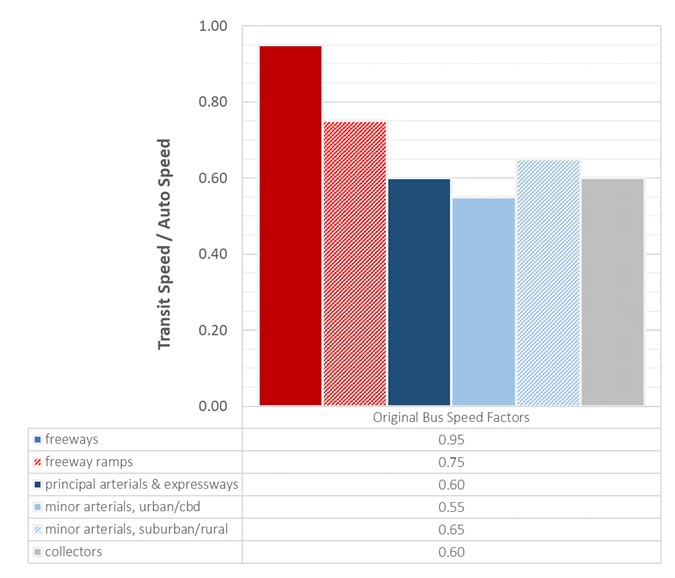
\includegraphics{v9x/v900/whats-new/_pictures/old_bus_speeds.png}

}

\caption{\label{fig-pdf-old-bus-speeds-plot}Bus Speeds Plot - Version
8.3.2}

\end{figure}

\begin{figure}[H]

{\centering 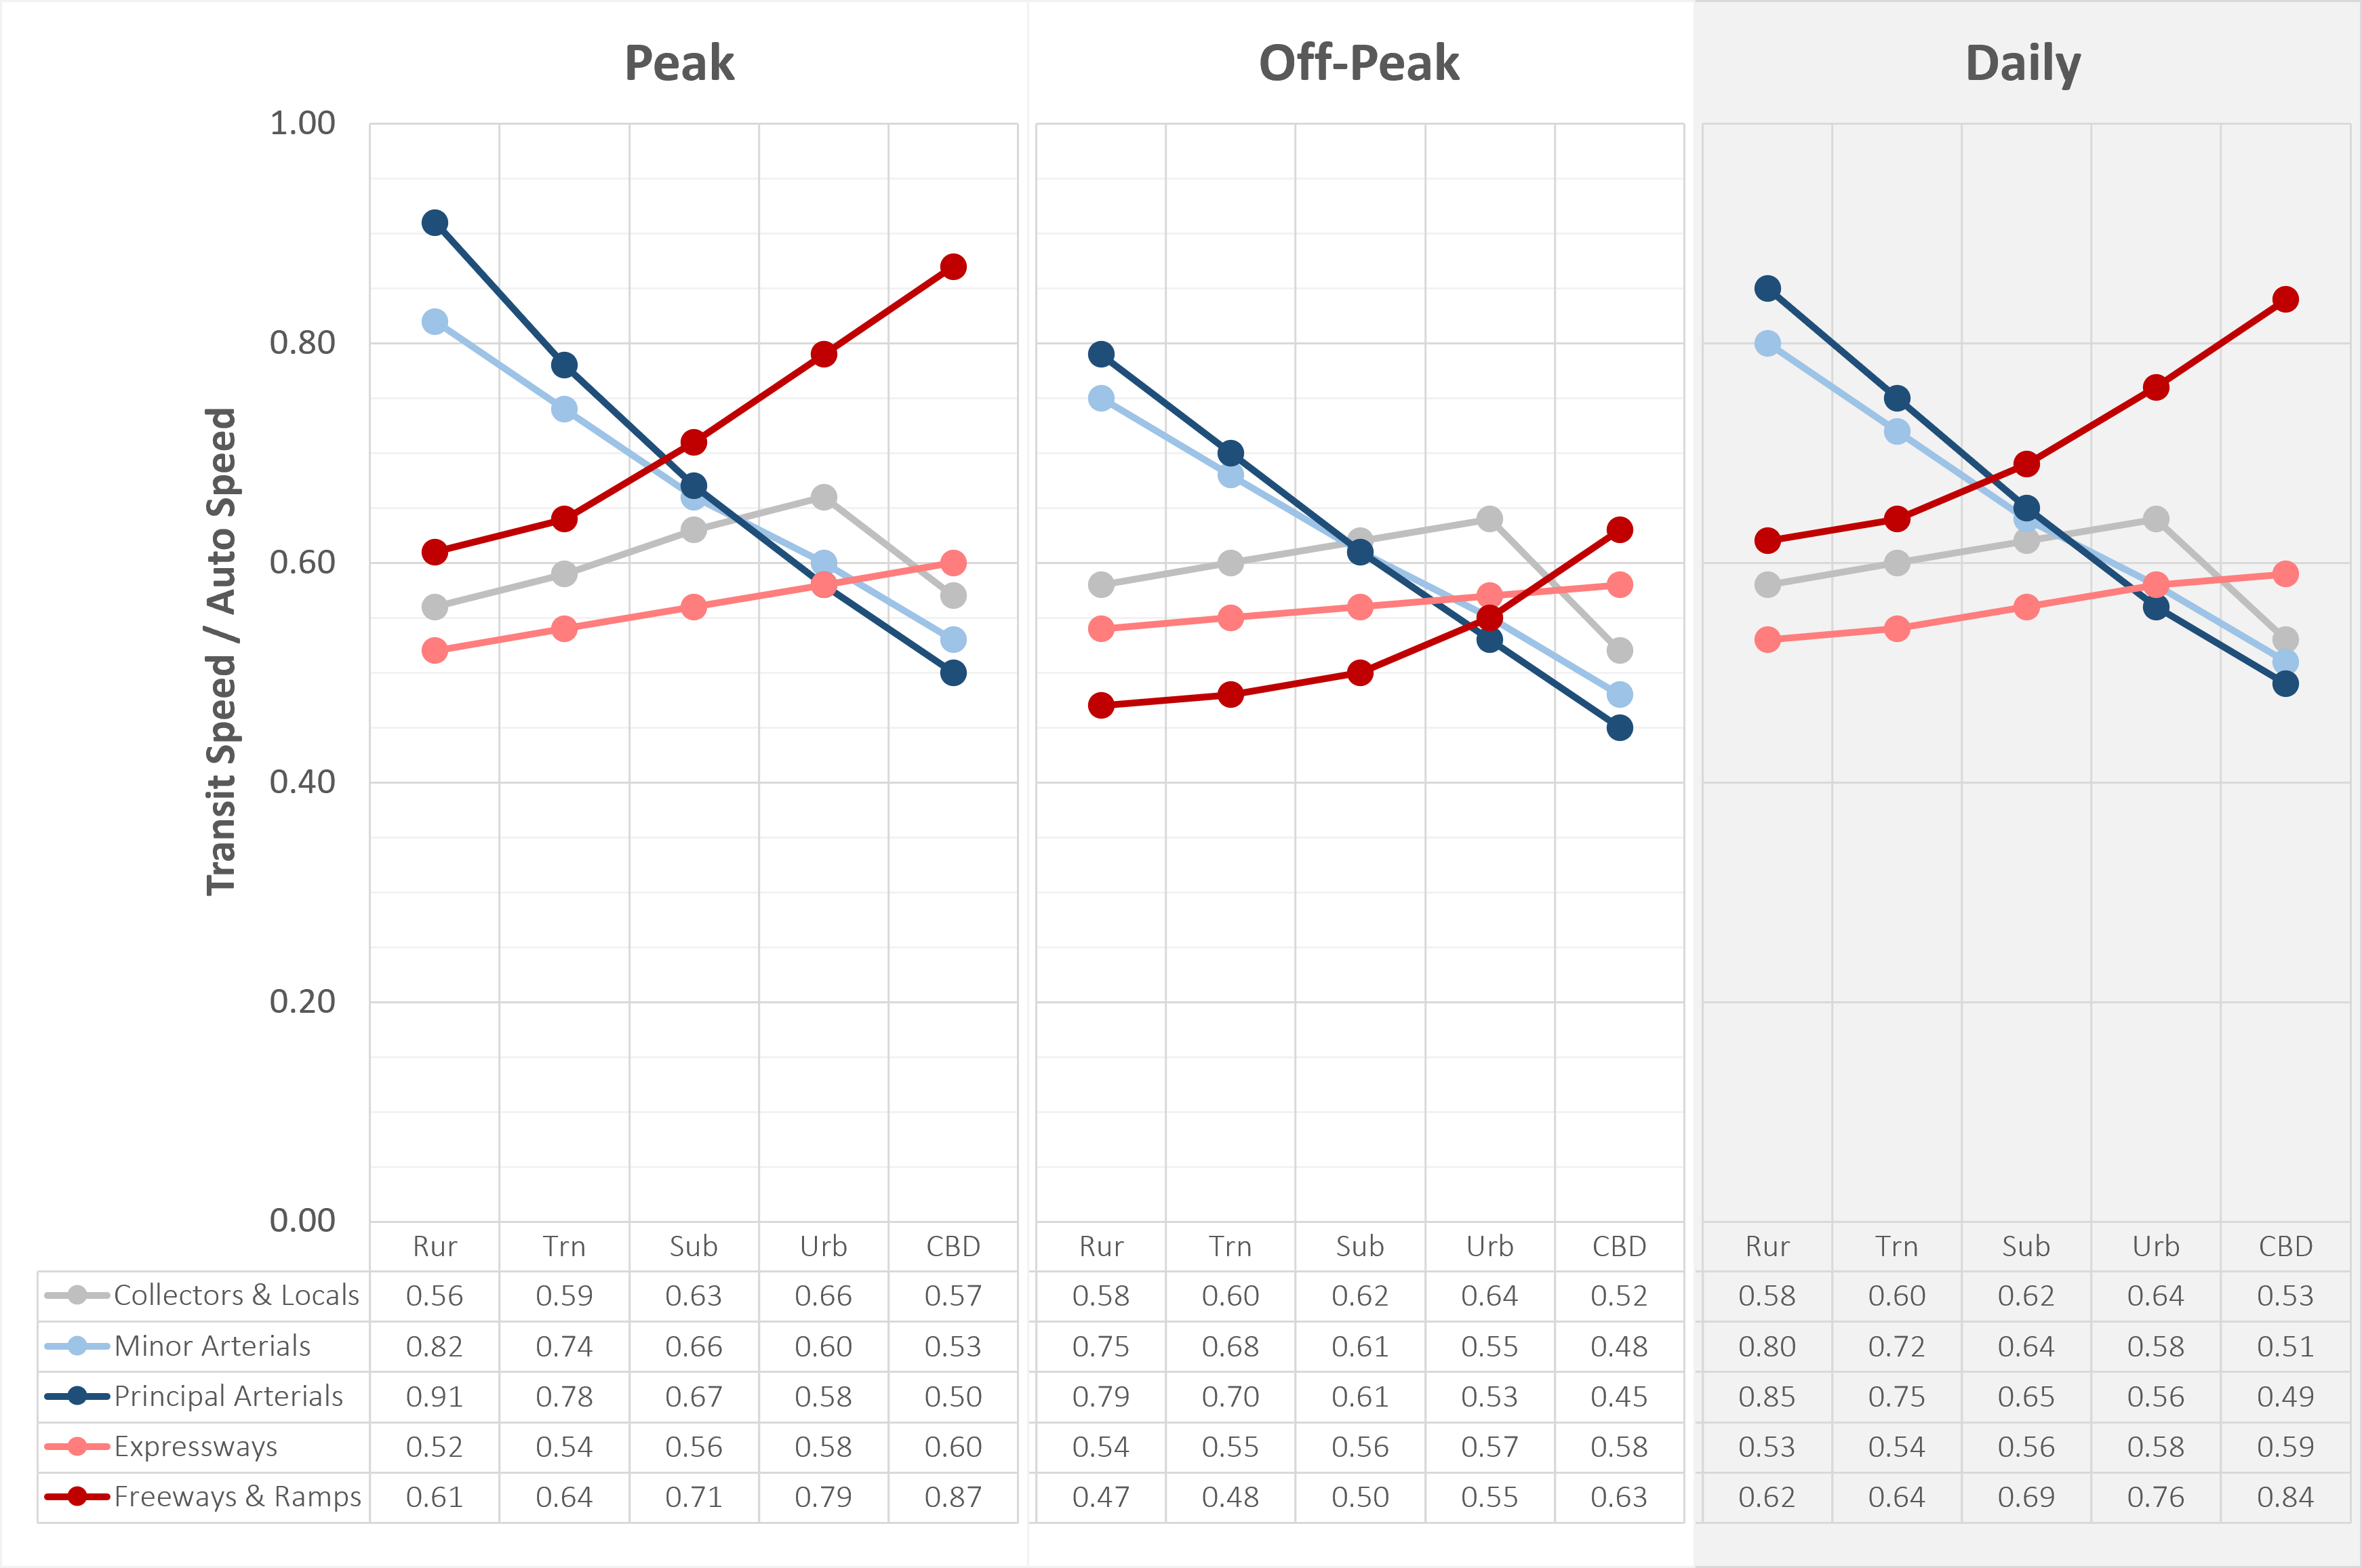
\includegraphics{v9x/v900/whats-new/_pictures/pdf-bus-speeds-plot.png}

}

\caption{\label{fig-pdf-bus-speeds-plot}Bus Speeds Plot - Version
9.0.0.}

\end{figure}

\newpage

\hypertarget{assignment}{%
\subsection{Assignment}\label{assignment}}

As described in the \emph{General Parameters} section, diurnal and
production/attraction factors were moved out of the
\texttt{0\_GeneralParameters.block} file to an input file. The factors
are now found in the \texttt{Diurnal\ \&\ PA\ factors.csv} file.

\hypertarget{traffic-analysis-zones-taz}{%
\section{Traffic Analysis Zones
(TAZ)}\label{traffic-analysis-zones-taz}}

\hypertarget{taz-geometry-geographic-changes}{%
\subsection{Taz Geometry \& Geographic
Changes}\label{taz-geometry-geographic-changes}}

TAZ geometry was updated and corrected. These updates include:

\begin{itemize}
\tightlist
\item
  Fixed the TAZ UTM NAD83 projection to use the standard for Utah rather
  than the ArcGIS default.
\item
  All TAZ boundaries align to county boundaries from the most current
  version on AGRC's website.
\item
  All internal TAZ topology was checked and corrected so there are no
  slivers, gaps, overlaps.
\end{itemize}

Internal zones were split to increase the model's geographic resolution.
Some zone boundaries were also modified without being split to better
align with underlying land uses and planning boundaries.

The geographic coverage area of the internal zones was also expanded to
encompass the entire county. The notable exceptions to this are the
portions of Box Elder County and Weber County that are not in the WFRC
planning domain. While not expanded to county boundaries, the geographic
coverage area of these counties was still changed to encompass the
canyon/mountain areas that are part of the Wasatch Front travel shed.

External zones were revised to reflect the changes of the expanded
internal zone area. This included an update to the number and location
of the external zones. However, external zones are no longer represented
in the TAZ shapefile. The arbitrary polygons representing the external
zones in previous version of the TAZ shapefile have been removed.
External zones are still represented in other parts of the model, such
as in the highway network, general parameters block file.

The expanded area and reconfigured TAZs resulted in the addition of 688
internal zones and 6 external zones. A comparison of zone counts is
found in Table~\ref{tbl-taz-count}.

\newpage

\begin{table}

\caption{\label{tbl-taz-count}TAZ Count
Comparisons}\begin{minipage}[t]{0.50\linewidth}
\subcaption{\label{tbl-internal}Internal}

{\centering 

\begin{tabular}[t]{llll}
\toprule
County & v9 & v832 & Change\\
\midrule
Box Elder & 153 & 135 & 18\\
Weber & 428 & 280 & 148\\
Davix & 324 & 231 & 93\\
Salt Lake & 1311 & 1127 & 184\\
Utah & 1330 & 1085 & 245\\
Total & 3546 & 2858 & 688\\
\bottomrule
\end{tabular}

}

\end{minipage}%
%
\begin{minipage}[t]{0.50\linewidth}
\subcaption{\label{tbl-external}External}

{\centering 

\begin{tabular}[t]{llll}
\toprule
County & v9 & v832 & Change\\
\midrule
Box Elder & 6 & 5 & 1\\
Weber & 3 & 3 & 0\\
Davix & 0 & 0 & 0\\
Salt Lake & 6 & 7 & -1\\
Utah & 14 & 8 & 6\\
Total & 29 & 23 & 6\\
\bottomrule
\end{tabular}

}

\end{minipage}%

\end{table}

The maps in Figure~\ref{fig-taz-compare-weber-pdf},
Figure~\ref{fig-taz-compare-davis-pdf},
Figure~\ref{fig-taz-compare-sl-pdf}, and
Figure~\ref{fig-taz-compare-utah-pdf} show the difference in version 9
and version 8 TAZs.

\begin{figure}[H]

{\centering 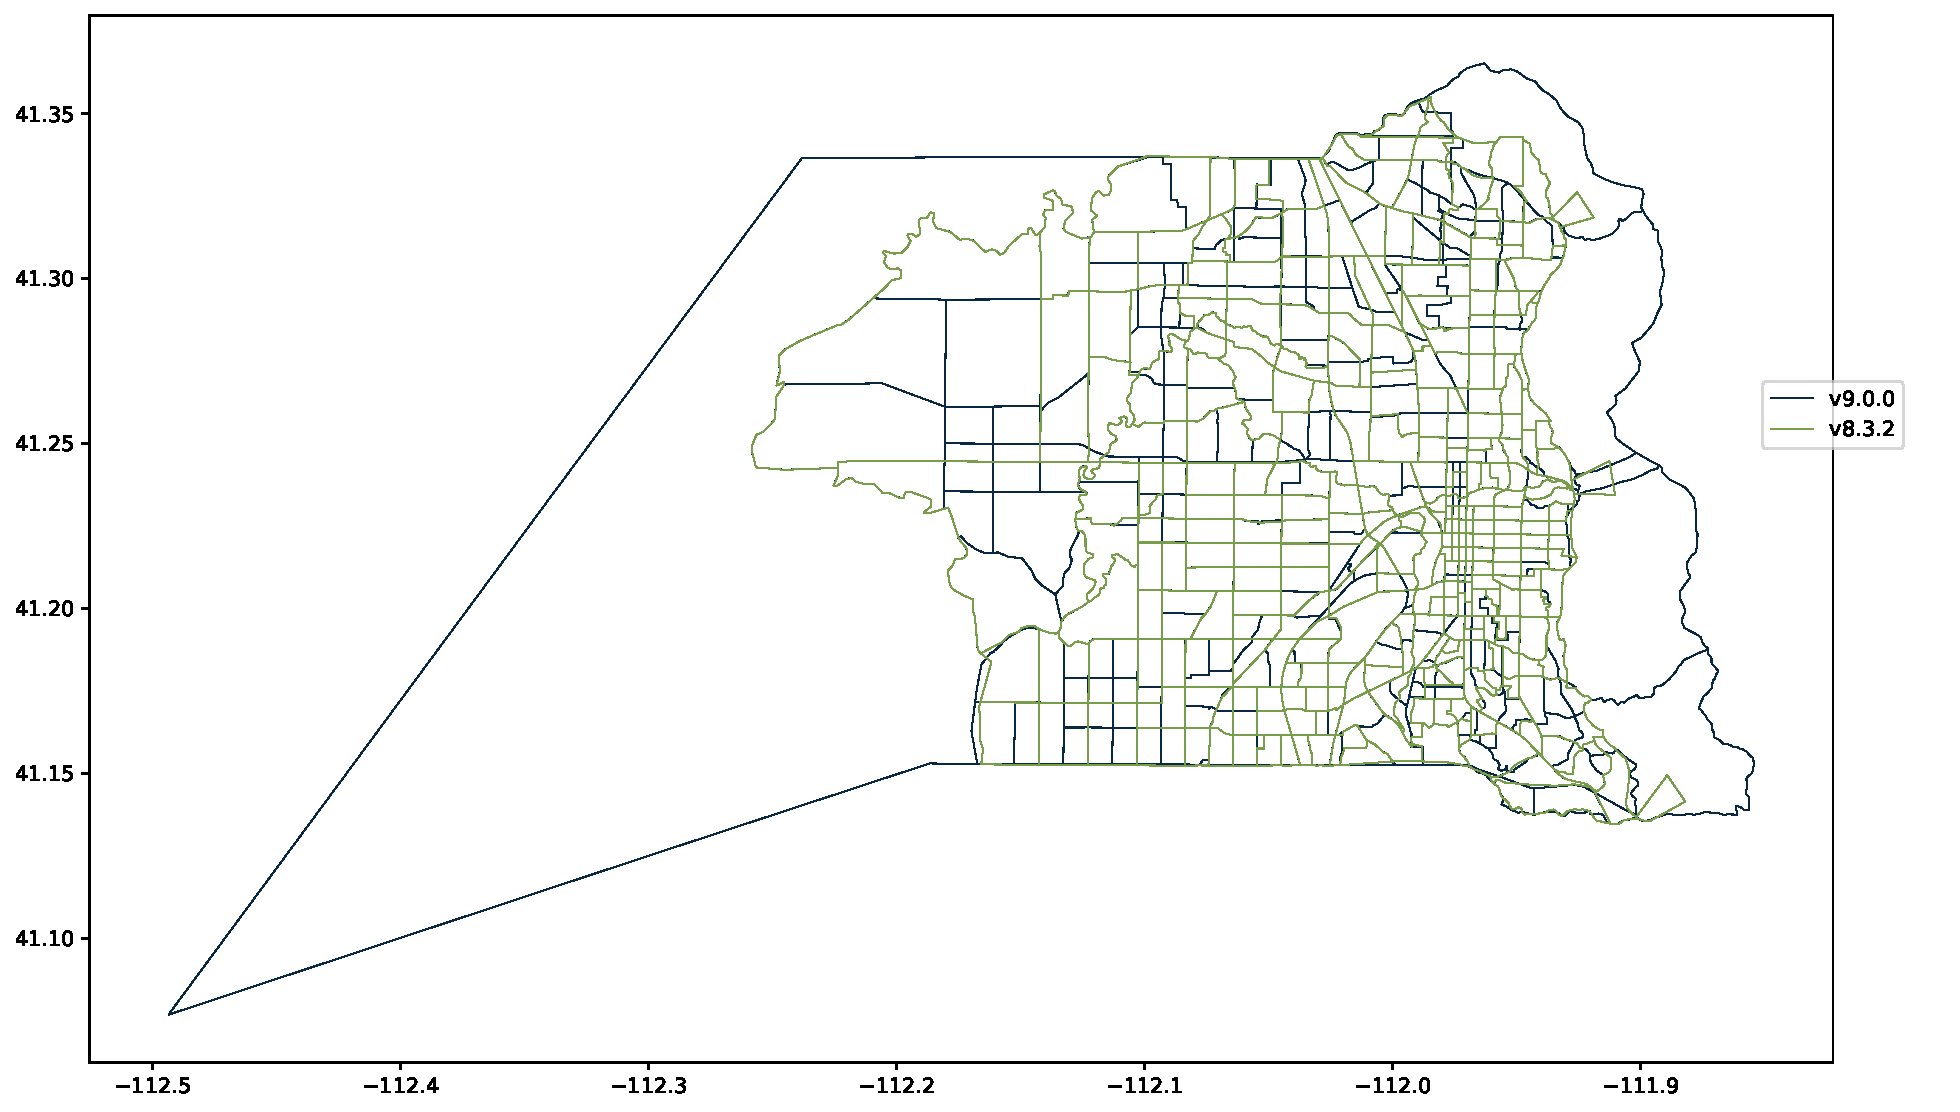
\includegraphics{v9x/v900/whats-new/2-inputdata_files/figure-pdf/fig-taz-compare-weber-pdf-output-1.pdf}

}

\caption{\label{fig-taz-compare-weber-pdf}TAZ Geography Comparison Map
-- Weber County}

\end{figure}

\begin{figure}[H]

{\centering 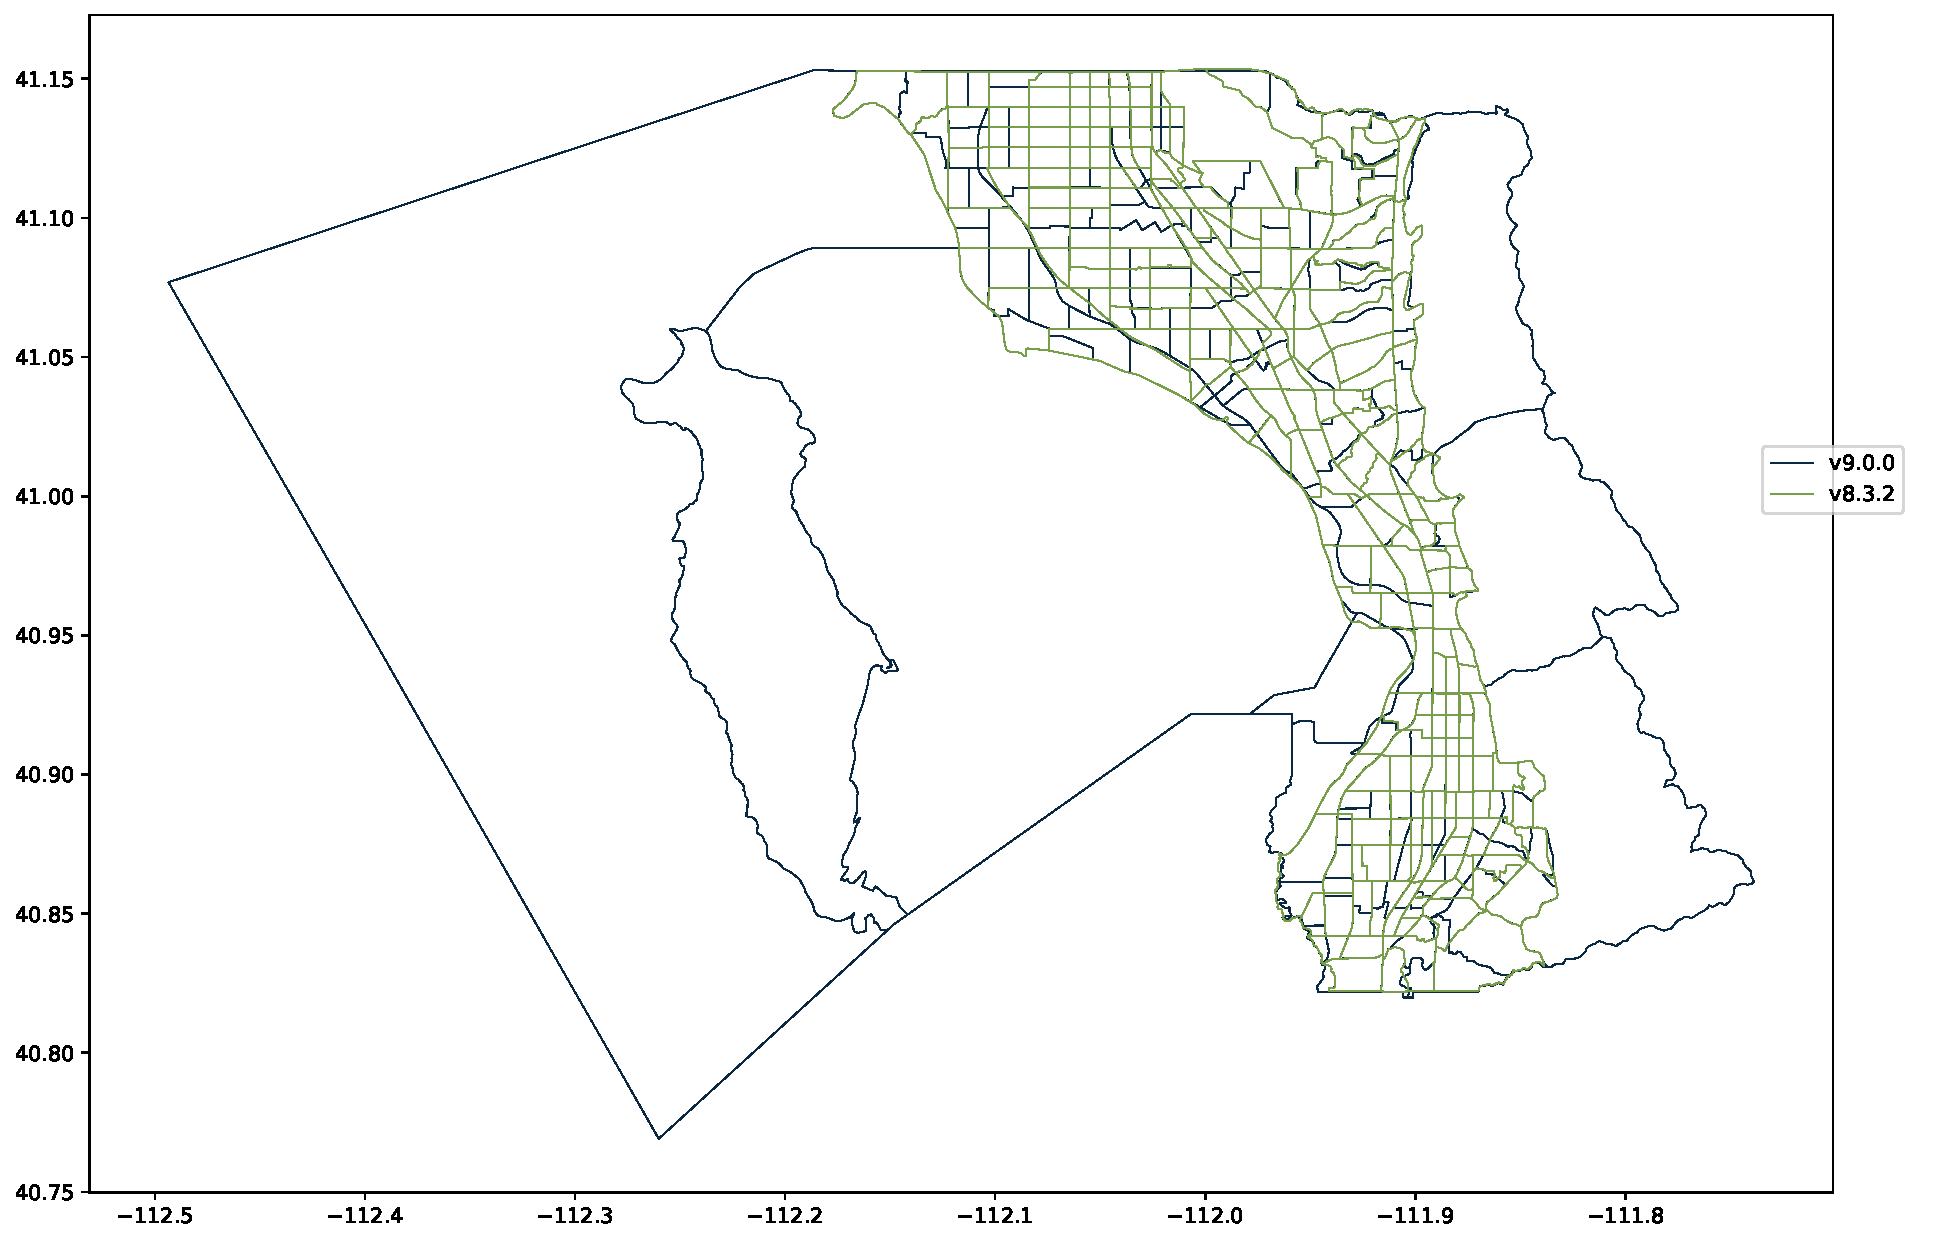
\includegraphics{v9x/v900/whats-new/2-inputdata_files/figure-pdf/fig-taz-compare-davis-pdf-output-1.pdf}

}

\caption{\label{fig-taz-compare-davis-pdf}TAZ Geography Comparison Map
-- Davis County}

\end{figure}

\begin{figure}[H]

{\centering 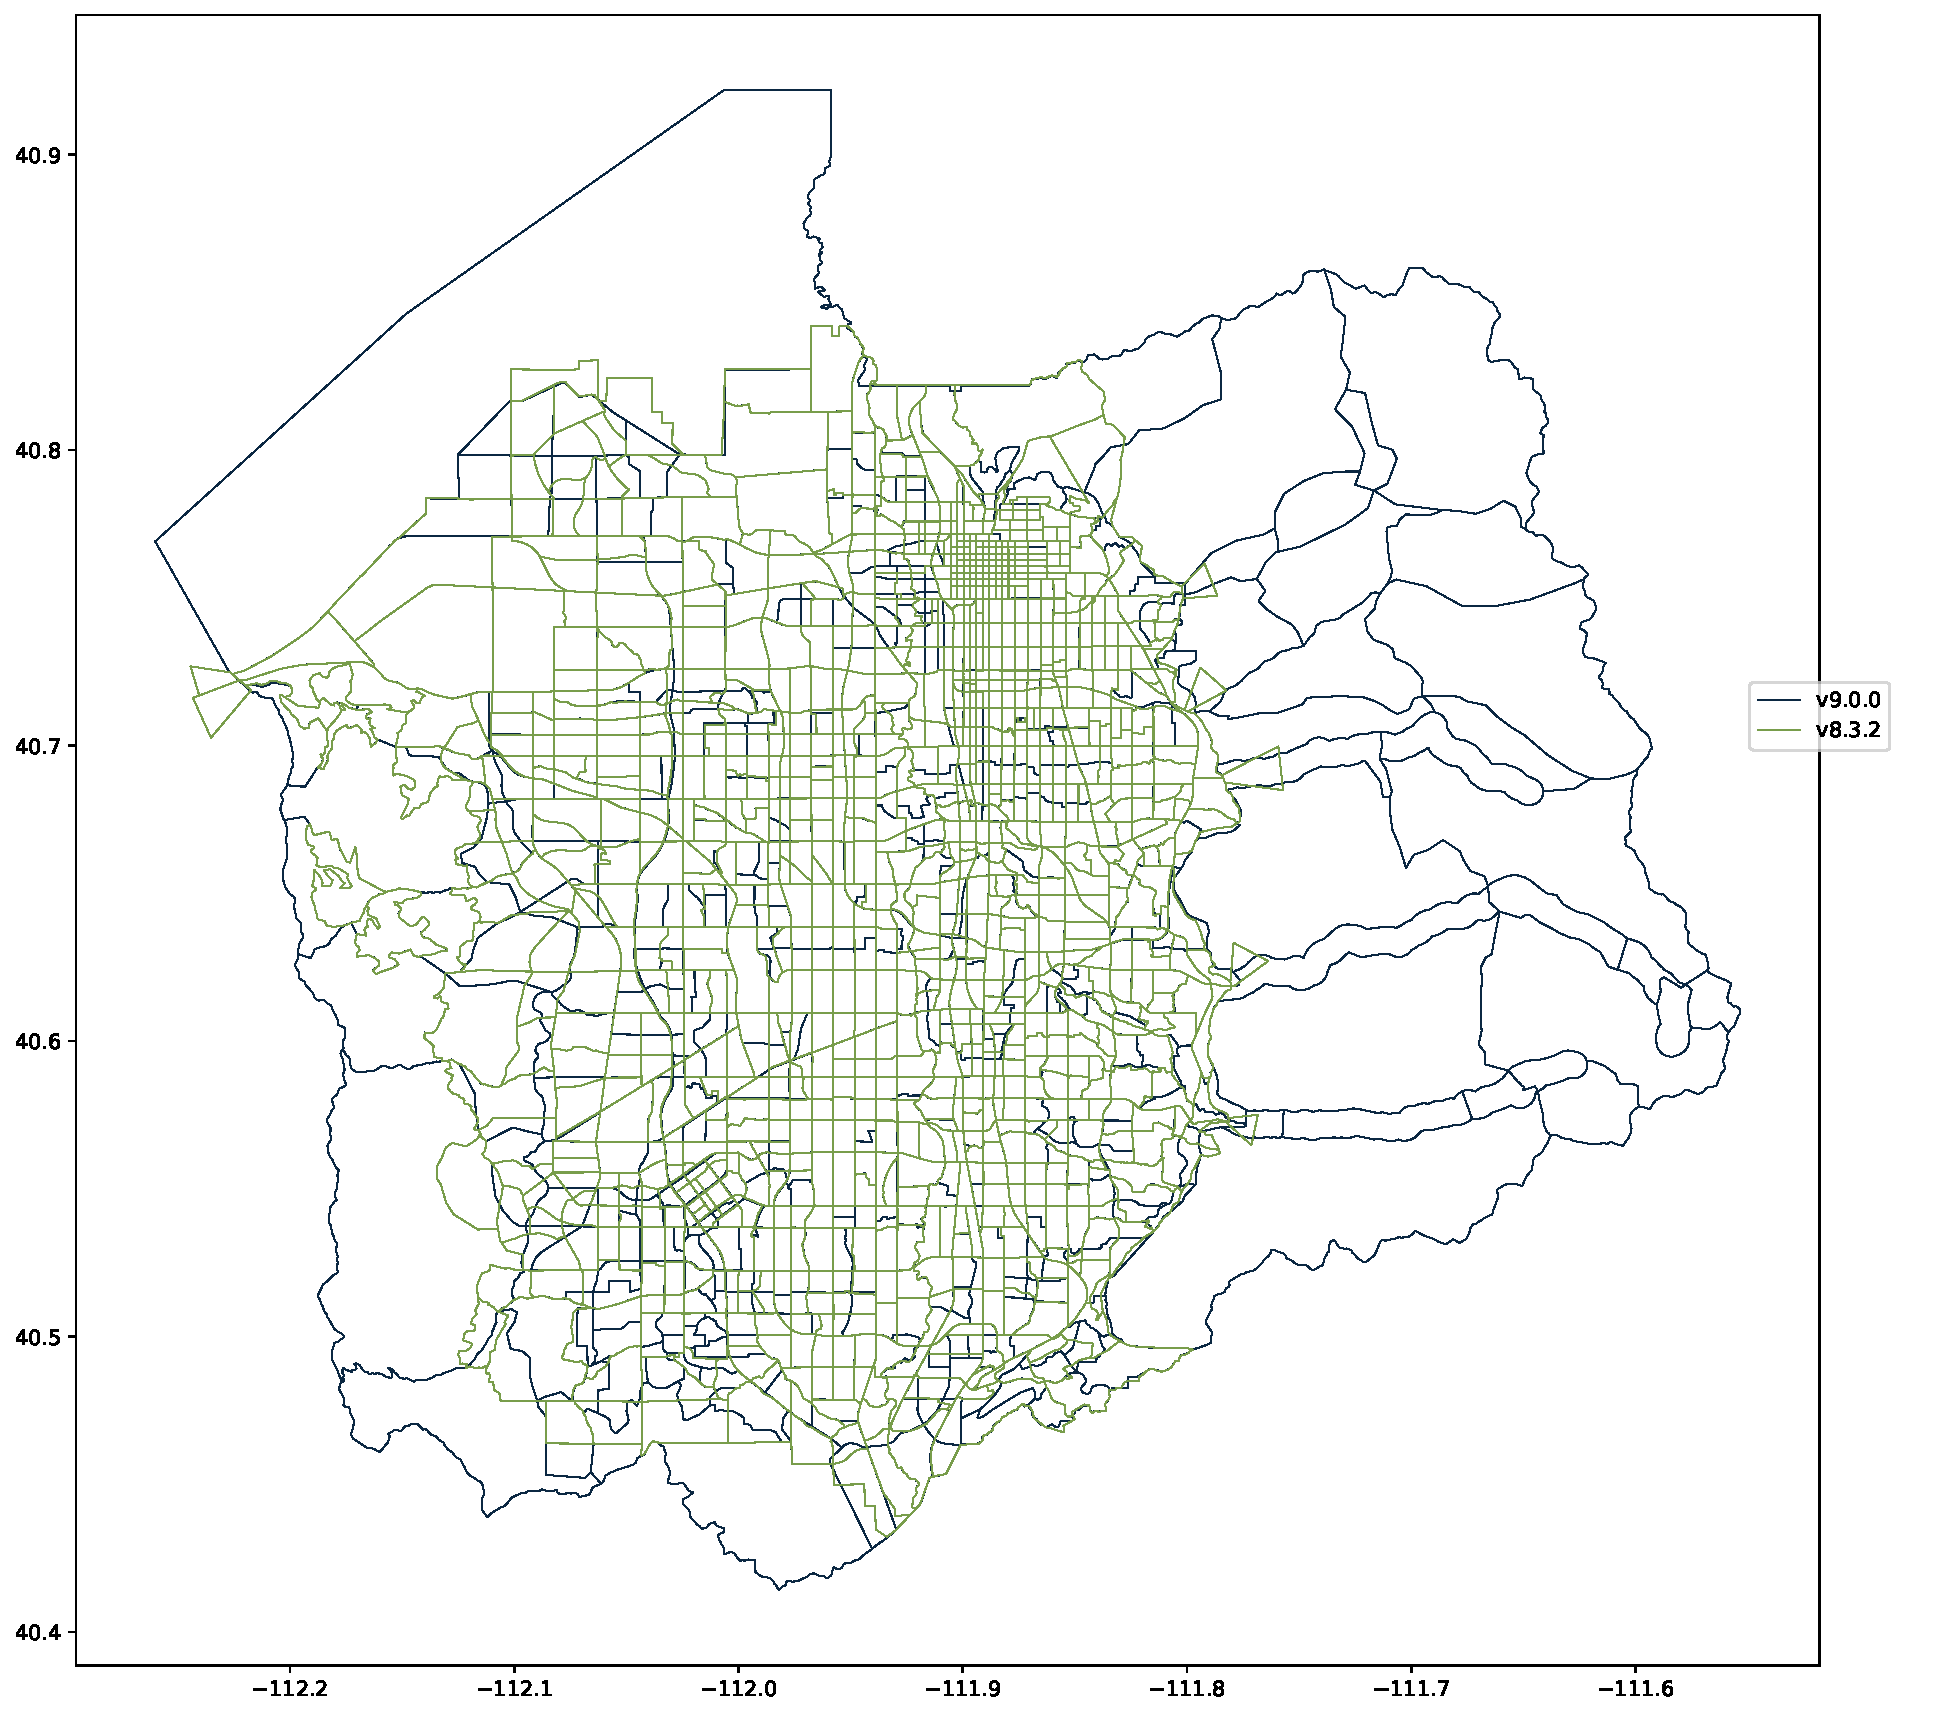
\includegraphics{v9x/v900/whats-new/2-inputdata_files/figure-pdf/fig-taz-compare-sl-pdf-output-1.pdf}

}

\caption{\label{fig-taz-compare-sl-pdf}TAZ Geography Comparison Map --
Salt Lake County}

\end{figure}

\begin{figure}[H]

{\centering 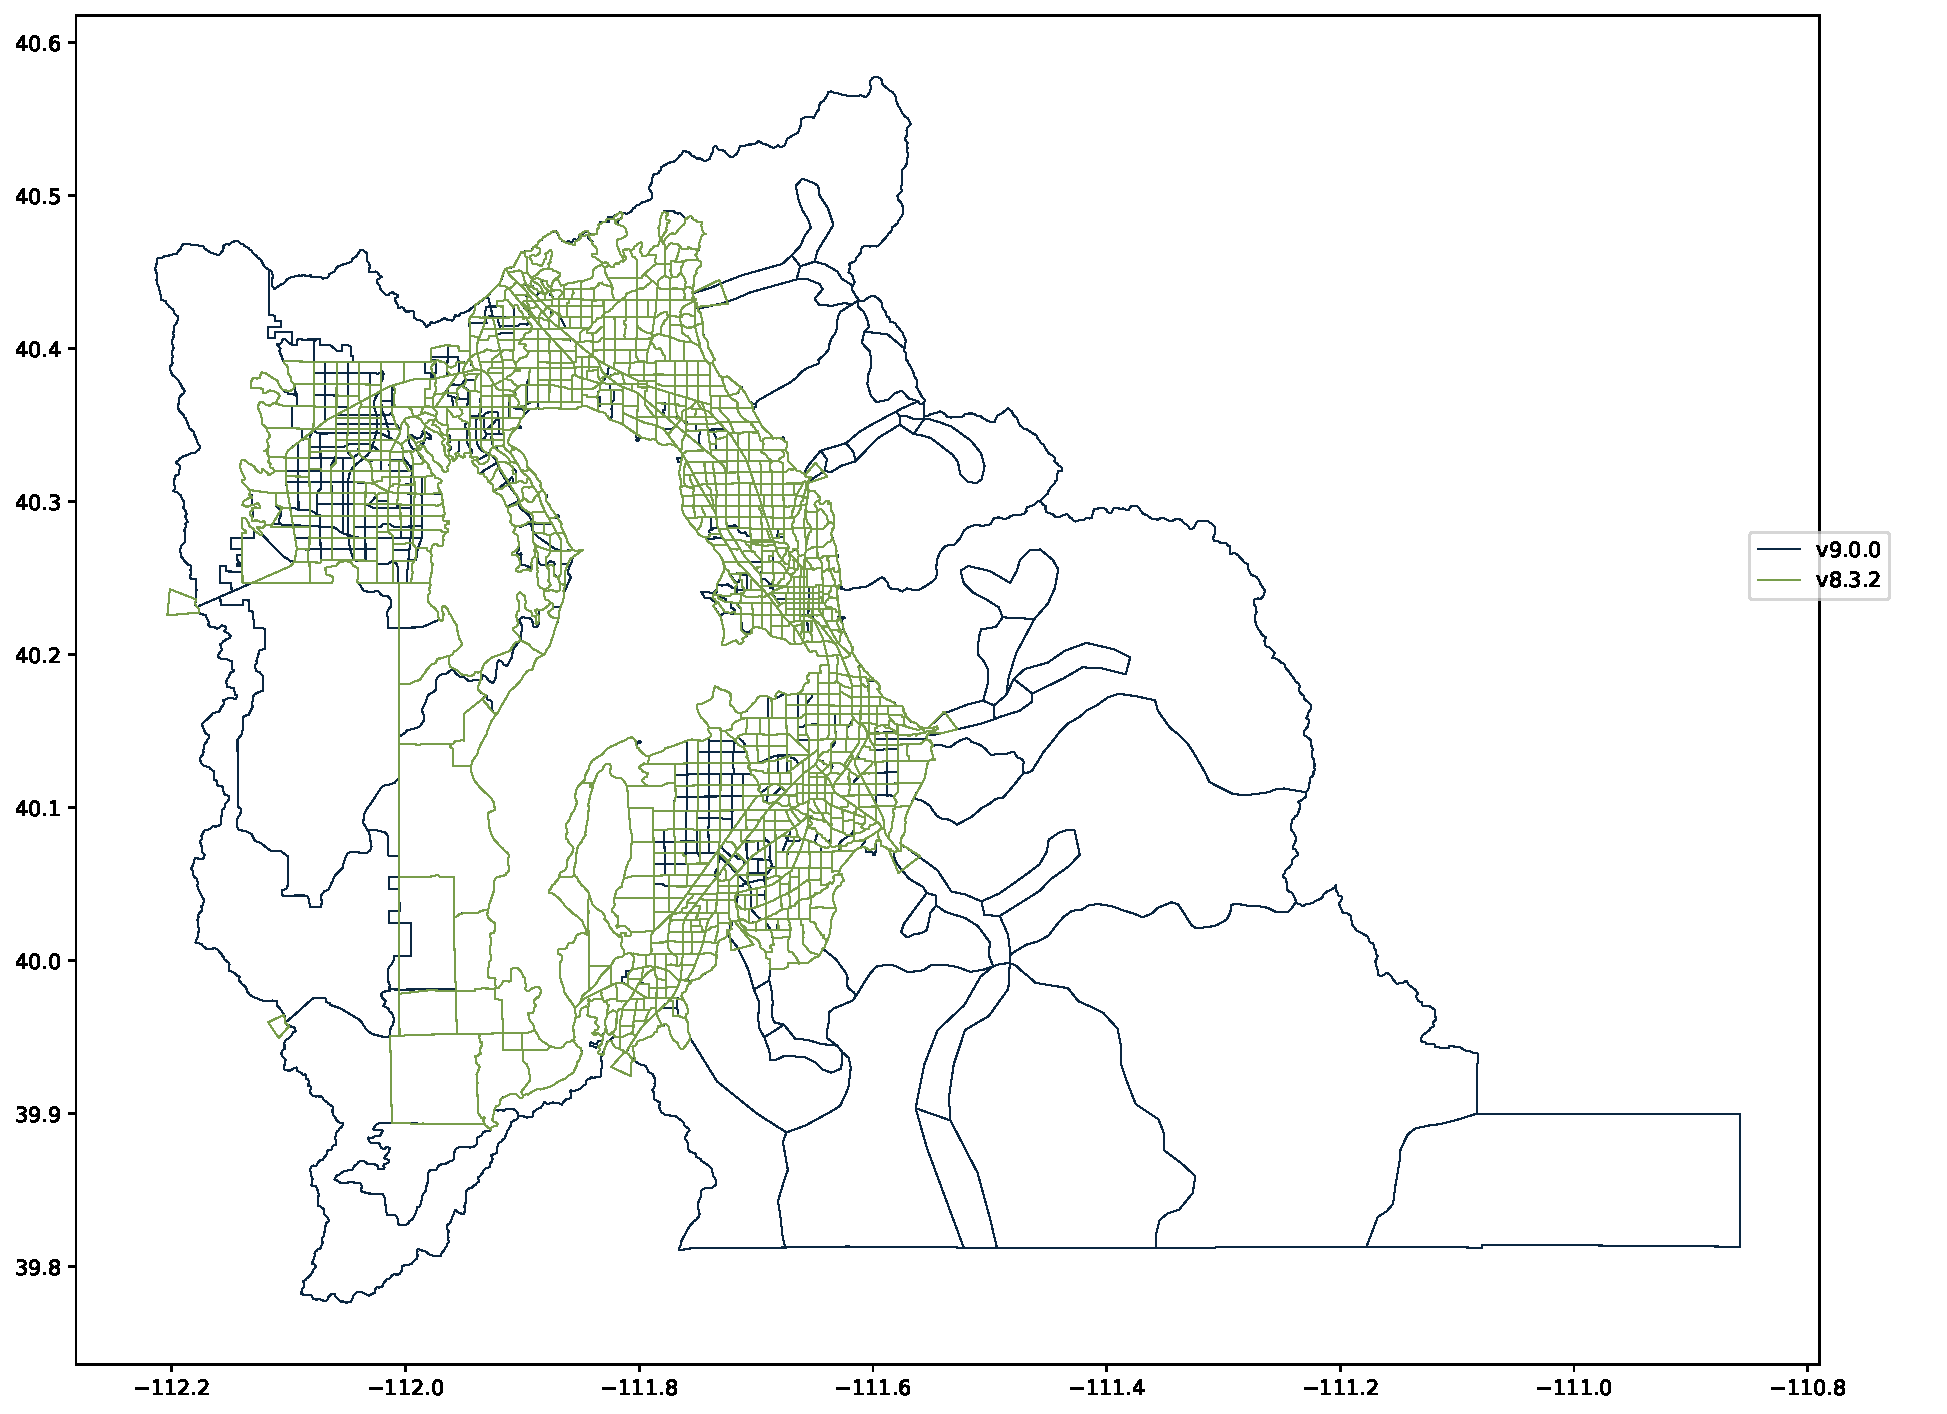
\includegraphics{v9x/v900/whats-new/2-inputdata_files/figure-pdf/fig-taz-compare-utah-pdf-output-1.pdf}

}

\caption{\label{fig-taz-compare-utah-pdf}TAZ Geography Comparison Map --
Utah County}

\end{figure}

The TAZ numbering was updated to reflect the changes made to the TAZ
geometry, as depicted in Table~\ref{tbl-new-taz-ranges}.

\hypertarget{tbl-new-taz-ranges}{}
\begin{longtable}[]{@{}
  >{\raggedright\arraybackslash}p{(\columnwidth - 8\tabcolsep) * \real{0.3700}}
  >{\raggedleft\arraybackslash}p{(\columnwidth - 8\tabcolsep) * \real{0.1600}}
  >{\raggedleft\arraybackslash}p{(\columnwidth - 8\tabcolsep) * \real{0.1600}}
  >{\raggedleft\arraybackslash}p{(\columnwidth - 8\tabcolsep) * \real{0.1600}}
  >{\raggedleft\arraybackslash}p{(\columnwidth - 8\tabcolsep) * \real{0.1600}}@{}}
\caption{\label{tbl-new-taz-ranges}TAZ Ranges}\tabularnewline
\toprule\noalign{}
\begin{minipage}[b]{\linewidth}\raggedright
County
\end{minipage} & \begin{minipage}[b]{\linewidth}\raggedleft
v9.0.0 Internal
\end{minipage} & \begin{minipage}[b]{\linewidth}\raggedleft
v9.0.0 External
\end{minipage} & \begin{minipage}[b]{\linewidth}\raggedleft
v8.3.2 Internal
\end{minipage} & \begin{minipage}[b]{\linewidth}\raggedleft
v8.3.2 External
\end{minipage} \\
\midrule\noalign{}
\endfirsthead
\toprule\noalign{}
\begin{minipage}[b]{\linewidth}\raggedright
County
\end{minipage} & \begin{minipage}[b]{\linewidth}\raggedleft
v9.0.0 Internal
\end{minipage} & \begin{minipage}[b]{\linewidth}\raggedleft
v9.0.0 External
\end{minipage} & \begin{minipage}[b]{\linewidth}\raggedleft
v8.3.2 Internal
\end{minipage} & \begin{minipage}[b]{\linewidth}\raggedleft
v8.3.2 External
\end{minipage} \\
\midrule\noalign{}
\endhead
\bottomrule\noalign{}
\endlastfoot
Box Elder County & 1-153 & 3601-3606 & 1-135 & 136-140 \\
Weber County & 154-581 & 3607-3609 & 141-420 & 421-423 \\
Davis County & 582-905 & N/A & 424-654 & N/A \\
Salt Lake County & 906-2216 & 3610-3615 & 655-1781 & 1782-1788 \\
Utah County & 2217-3546 & 3616-3629 & 1789-2873 & 2874-2881 \\
\end{longtable}

\hypertarget{taz-attribute-changes}{%
\subsection{TAZ Attribute Changes}\label{taz-attribute-changes}}

This section describes the changes made to the attributes of the TAZ
shapefile.

\hypertarget{remm-space}{%
\subsubsection{REMM Space}\label{remm-space}}

To indicate which TAZs are included in the Real Estate Market Model
(REMM) space, the \texttt{REMM} field was added with a value of
\texttt{1} indicating that it is part of REMM and \texttt{0} indicating
it is not part of REMM, as shown in Figure~\ref{fig-taz-remm-space-pdf}.

\begin{figure}[H]

{\centering 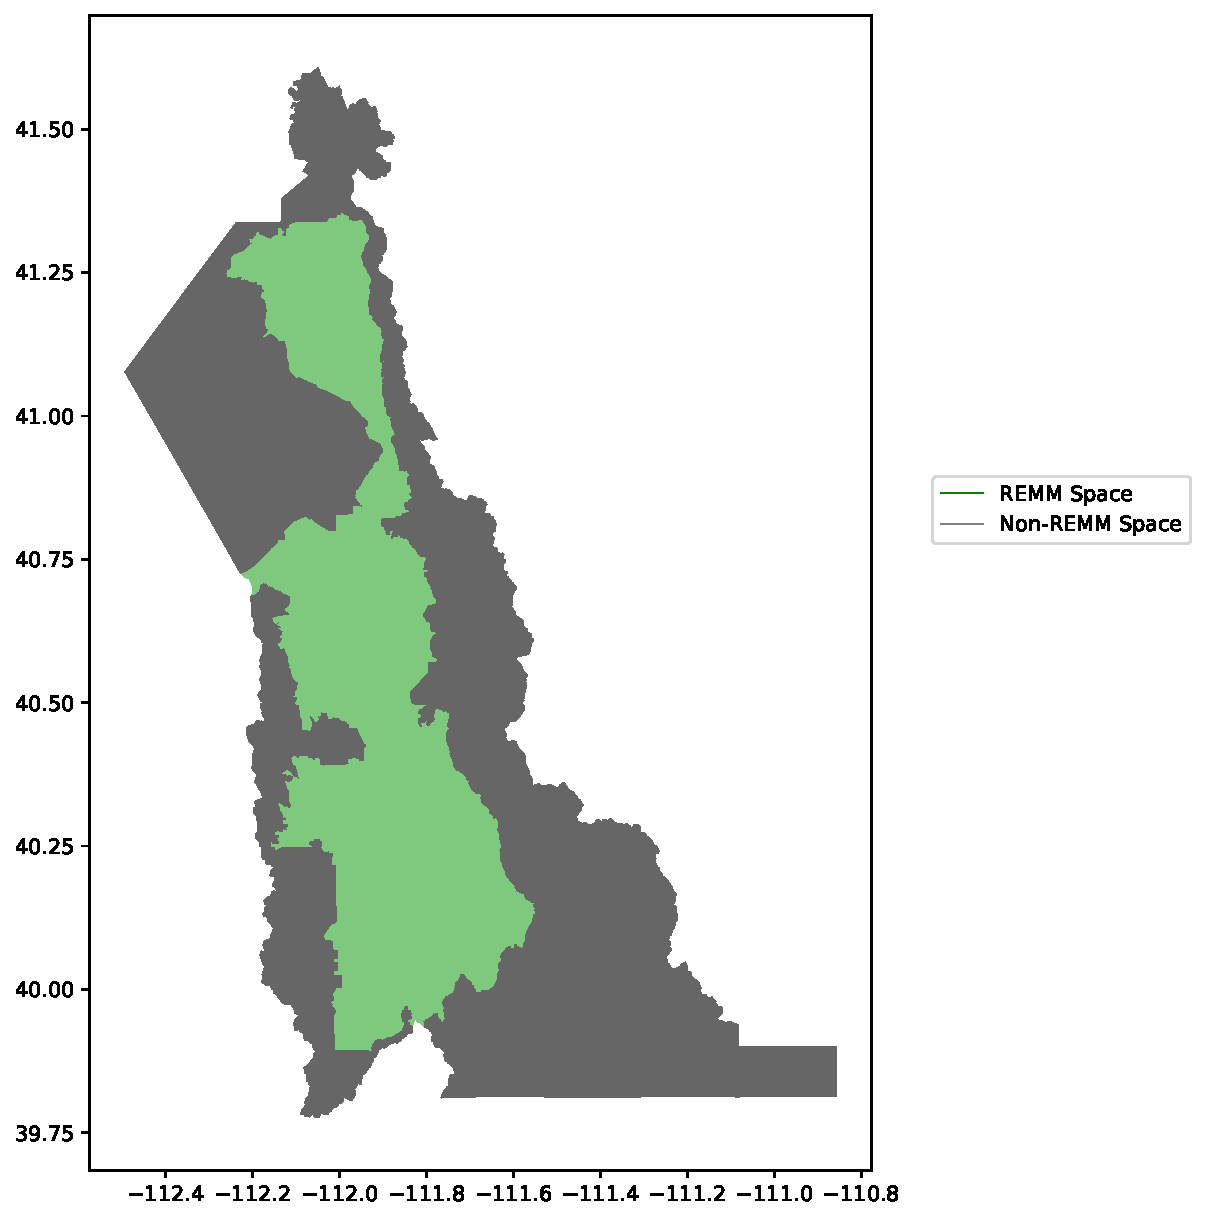
\includegraphics{v9x/v900/whats-new/2-inputdata_files/figure-pdf/fig-taz-remm-space-pdf-output-1.pdf}

}

\caption{\label{fig-taz-remm-space-pdf}TAZ REMM Space}

\end{figure}

\hypertarget{parking-costs}{%
\subsubsection{Parking Costs}\label{parking-costs}}

Parking costs were updated based on 2022 parking rates obtained from
Salt Lake City, web searches, and field visits. A new methodology for
calculating parking cost was envisioned but not implemented for v9.
Accordingly, updates to parking data were done in a way to facilitate
the change to the new methodology in the future. These updates include a
new polygon source file for downtown and university areas. However,
since the envisioned methodology removes the use of parking cost fields
for Lagoon and Salt Lake City International Airport, they were not
included in this new shapefile.

\hypertarget{downtown-and-university-areas}{%
\paragraph{Downtown and University
Areas}\label{downtown-and-university-areas}}

Parking costs were developed for downtown areas for Ogden, Salt Lake
City, and Provo, as well as major university areas along the Wasatch
Front. A new source polygon shapefile was developed to hold rates for
Home-Based Work (HBW), Home-Based College (HBC), Home-Based Other (HBO),
and Non-Home-Based (NHB) trip purposes. While rates are included for
these four purposes, the v9.0.0 model only utilizes HBW for permanent
parking and HBO for temporary parking. The future methodology will
incorporate all four purposes.

\hypertarget{lagoon-and-salt-lake-city-international-airport}{%
\paragraph{Lagoon and Salt Lake City International
Airport}\label{lagoon-and-salt-lake-city-international-airport}}

The Airport \& Lagoon parking costs were updated based on current
parking rate information and the assumptions described in this section.

The cost of permanent parking for the Lagoon TAZ was set to \texttt{\$0}
based on the assumption that workers at Lagoon do not pay for parking.
The temporary parking was set to \texttt{\$6} as calculated by dividing
the 2022 advertised parking rate of \$18 per day by an assumed average
occupancy of 3 people per vehicle. The cost of temporary parking in
previous models was \$5 in 2010 dollars. The resulting \$1 increase in
2019 dollars (20\%) over 9 years seems reasonable.

The cost of permanent parking at the Salt Lake City International
Airport was set to \emph{\$0} based on the assumption that workers at
the airport do not pay for parking. The cost of temporary parking was
set to \$1.25 based on a weighted average of short-term premium and
economy rates and drop offs and a assumed average vehicle occupancy
rate.

The 2022 the cost for the short-term premium parking in the garage is
\$5.00 per hour. Short-term economy rate is \$2.00 per hour. And for
drop-offs there is no charge for parking. The assumed occupancy rate of
2 people per vehicle would result in per-person rates of \$2.50, \$1.00,
and \$0.00, respectively. The average of the three per-person rates is
\$1.75. Given the unknown distribution of travelers, but assuming more
drop-offs than parking, a lower value than \$1.75 should be expected.
The 2019 cost was chosen to be \$1.25.

Compared to the previous temporary parking values of \$1 in 2010
dollars, the chosen cost represents a 25 cent increase in 2019 dollars
(25\%) over 9 years. This growth seems reasonable, especially given the
recent improvements to the airport. Additional justification for the
chosen increase is the
\href{https://www.bls.gov/data/inflation_calculator.html}{CPI
adjustment}, which for the 2010 value of \$1.00 in results in a 2019
value of \$1.18.

\hypertarget{small-districts}{%
\subsection{Small Districts}\label{small-districts}}

There are now 129 total small districts sequentially numbered from
northwest to southeast in each medium district. The small district name
field \texttt{DSML\_NAME} includes a prefix of Medium District index
followed by a colon and then the sequential small district count
(e.g.~15:1). Districts are shown in Figure~\ref{fig-districts-pdf}. Two
additional polygon shapefiles were added to the Districts subfolder to
represent the Wasatch Front sub area and the REMM area.

\begin{figure}[H]

{\centering 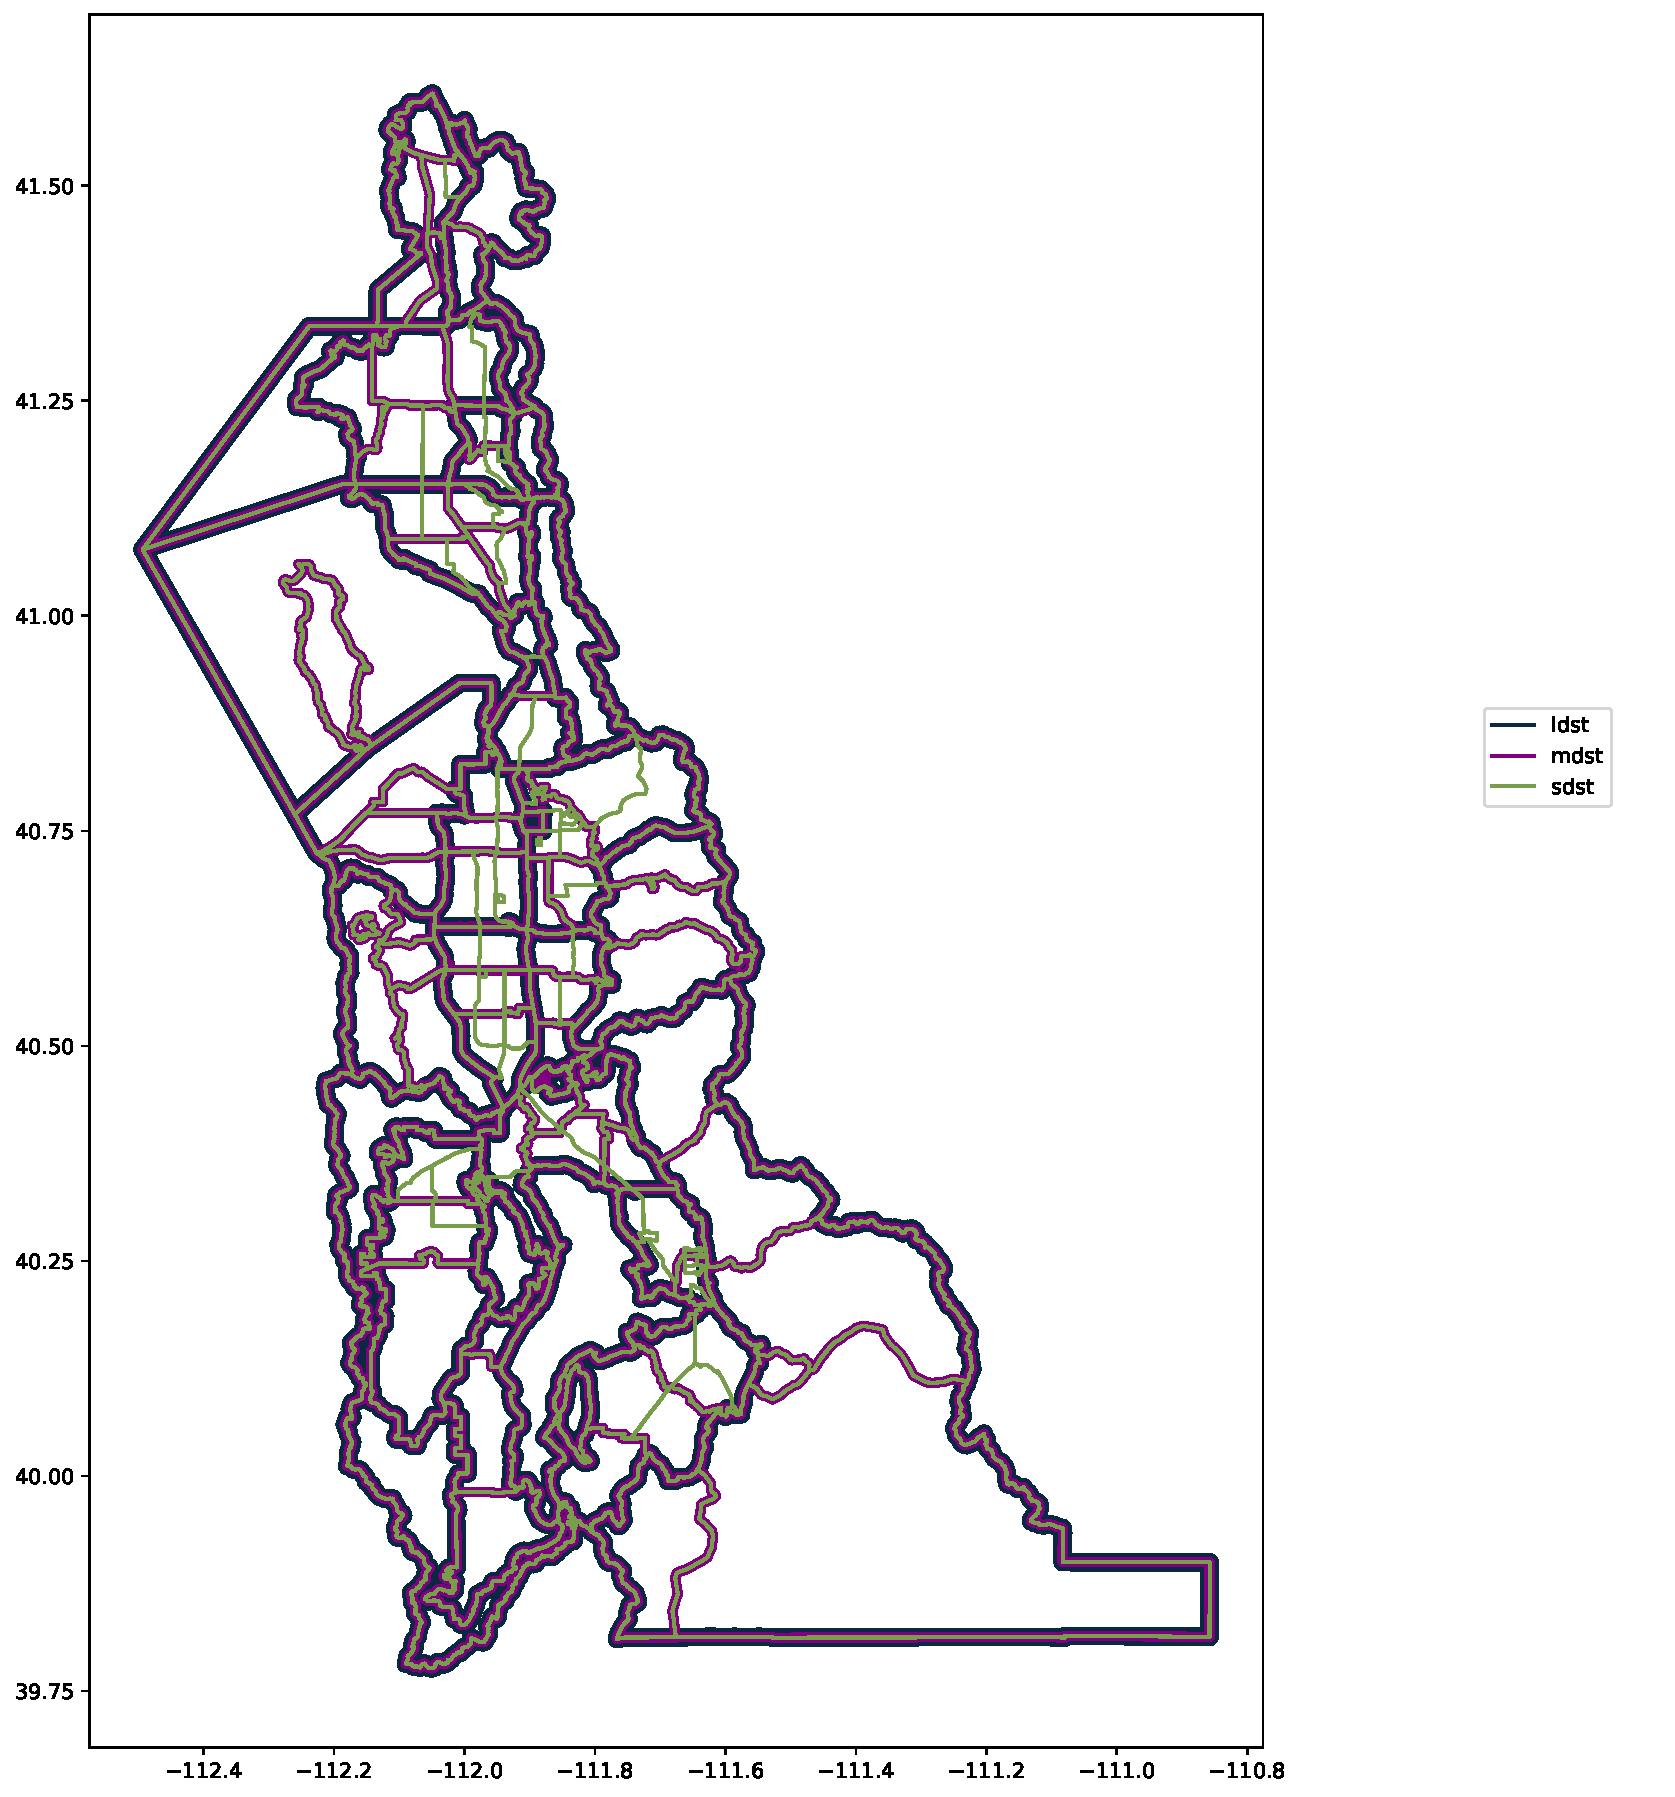
\includegraphics{v9x/v900/whats-new/2-inputdata_files/figure-pdf/fig-districts-pdf-output-1.pdf}

}

\caption{\label{fig-districts-pdf}Districts}

\end{figure}

\hypertarget{source}{%
\subsection{Source}\label{source}}

The \texttt{\_Source} subfolder was added and includes the following
shapefile data sets: Cities, Counties, Districts, and Environmental
Constraints. Additionally, a ArcGIS Pro project \& mapping files can be
found in the \texttt{\_\_ViewTAZDistricts} subfolder.

\hypertarget{socioeconomic-data}{%
\section{Socioeconomic Data}\label{socioeconomic-data}}

Forecasts and control totals were updated based on new census data,
updated base year parcel data, and the results of the REMM Model.

\hypertarget{forecasts}{%
\subsection{Forecasts}\label{forecasts}}

The SE forecasts were updated for the WFRC areas. Box Elder updates were
taken from the UDOT SE Forecasts from June 8, 2022. The updated SE
forecasts can be found using the
\href{https://wfrc.org/household-job-forecast-map}{Household and Job
Forecasts Web App}. This map only contains the latest forecast and not
any iterative step, such as the SE datasets in the model folder. Click
on the \emph{View Advanced Version} link in the header to enable the
``Changes'' option where you can see the change in forecasts between
v8.3.2 and v9.0.0.

\hypertarget{control-totals}{%
\subsection{Control Totals}\label{control-totals}}

Updates to the county control totals were made based on projections from
the Gardner Policy Institute.

\hypertarget{school-enrollment}{%
\subsection{School Enrollment}\label{school-enrollment}}

The Kindergarten through 12th grade (K-12) enrollment data was updated
using the 2019 statewide school enrollment database. This was done at
the state-wide level and then applied to the Wasatch Front.

\hypertarget{median-income}{%
\subsection{Median Income}\label{median-income}}

Median income \& value-of-time (VOT) inputs for the model were updated
with 2019 data and used to update the TAZ Median Income in the TAZ file.

\hypertarget{highway-network}{%
\section{Highway Network}\label{highway-network}}

The highway network was expanded to incorporate the new model areas. See
TAZ Geographies. The 2023 RTP fields have been updated to reflect the
adopted 2023 RTP.

\hypertarget{highway-node-numbering-schema}{%
\subsection{Highway Node Numbering
Schema}\label{highway-node-numbering-schema}}

Updates to the highway node numbering schema are shown in
Table~\ref{tbl-master-network-node-numbering-schema}. An additional
reference file called \texttt{\_Node\ Definition\ -\ v832\ \&\ v9.xlsx}
is found in the \texttt{3\_Highway} folder.

\hypertarget{tbl-master-network-node-numbering-schema}{}
\begin{longtable}[]{@{}
  >{\raggedright\arraybackslash}p{(\columnwidth - 6\tabcolsep) * \real{0.4400}}
  >{\raggedright\arraybackslash}p{(\columnwidth - 6\tabcolsep) * \real{0.1900}}
  >{\raggedright\arraybackslash}p{(\columnwidth - 6\tabcolsep) * \real{0.1900}}
  >{\raggedright\arraybackslash}p{(\columnwidth - 6\tabcolsep) * \real{0.1900}}@{}}
\caption{\label{tbl-master-network-node-numbering-schema}Master Network
Node Numbering Schema}\tabularnewline
\toprule\noalign{}
\begin{minipage}[b]{\linewidth}\raggedright
MPO
\end{minipage} & \begin{minipage}[b]{\linewidth}\raggedright
Transit Nodes
\end{minipage} & \begin{minipage}[b]{\linewidth}\raggedright
Highway Nodes
\end{minipage} & \begin{minipage}[b]{\linewidth}\raggedright
v9 Expansion Areas
\end{minipage} \\
\midrule\noalign{}
\endfirsthead
\toprule\noalign{}
\begin{minipage}[b]{\linewidth}\raggedright
MPO
\end{minipage} & \begin{minipage}[b]{\linewidth}\raggedright
Transit Nodes
\end{minipage} & \begin{minipage}[b]{\linewidth}\raggedright
Highway Nodes
\end{minipage} & \begin{minipage}[b]{\linewidth}\raggedright
v9 Expansion Areas
\end{minipage} \\
\midrule\noalign{}
\endhead
\bottomrule\noalign{}
\endlastfoot
WFRC & 10,000 - 19,999 & 20,000 - 49,999 & 90,000 - 94,999 \\
MAG & 50,000 - 59,999 & 60,000 - 89,999 & 95,000 - 99,999 \\
\end{longtable}

The highway network updates include the following:

\begin{itemize}
\tightlist
\item
  Updated Commuter-Rail Transit (CRT) Fare Zone

  \begin{itemize}
  \tightlist
  \item
    Vineyard \& Orem stations were modified to have the same fare zone
    (similar to North Temple \& Central)
  \item
    Updated and fixed fare zone definitions in WFRC area
  \end{itemize}
\item
  Fixed small network error in Box Elder where a local road was drawn to
  the centroid of v8.3.2 TAZ 53
\item
  A few edits to WFRC draft RTP project list
\item
  Updated segment ids

  \begin{itemize}
  \tightlist
  \item
    Made consistent with the latest segment shapefile
  \item
    Updated segments to account for recent network changes \& add
    segment definitions to account for rail transit
  \end{itemize}
\item
  Added \texttt{SEGEX\_RTP} \& \texttt{SEGEX\_NEED} as text fields (to
  be populated later when script/processing updated). These are segment
  ID exception fields where the future SEGIDs are different than
  existing SEGIDs.
\item
  Phase change for Managed Motorways in WFRC area
\item
  A couple of phasing updates from the WFRC RTP project list
\item
  Cleaned up \texttt{GIS23\_32} and \texttt{GIS23\_42} fields
\item
  Differentiated what projects will be built by 2028 from what will be
  built by 2023
\item
  Rail \texttt{SEGID} additions were made to allow for easier transit
  result visualization.
\end{itemize}

Additionally, a \texttt{MergedMasterNet\ -\ 2022-09-19a} folder was
added to serve as a workspace for editing and updating Merged Master
Network and for exporting to v8.3.2 \& v9 master networks.

\hypertarget{transit}{%
\section{Transit}\label{transit}}

The transit line files and CUBE Public Transport (PT) files were updated
to correspond with the 2023 RTP:

\begin{itemize}
\tightlist
\item
  2019 was thoroughly vetted to represent Aug 2019 change day
\item
  2023: updated route alignment, headways \& stops based on August 2022
  change day (WFRC \& MAG)
\item
  2028: updated route alignment, headways \& stops based on UTA 5-Year
  Service Plan (WFRC \& MAG)
\item
  RTP 2032, 2042 \& 2050: rolled 2028 changes forward into plan phased
  years \& updated based on 2023 draft plan
\item
  Needs 2032, 2042 \& 2050: rolled 2028 changes forward into plan phased
  years \& updated based on 2023 draft plan
\end{itemize}

Route S902 was updated so route no longer go to the I-80 Parleys Canyon
external node.

\hypertarget{public-transport-pt-parameters}{%
\subsection{Public Transport (PT)
Parameters}\label{public-transport-pt-parameters}}

The fare files were updated with 2019 fare data. The fares were updated
to match the actual advertised fares, whereas the v8.3.2 model contained
a 46\% adjustment fares. This reduction accounts for monthly pass,
education, fare-pay, senior, employer paid, and other discounts. This
adjustment is now explicitly defined, as was discussed in the
\emph{General Parameters} section.

\hypertarget{general-hand-coded-support-links}{%
\subsection{General Hand-Coded Support
Links}\label{general-hand-coded-support-links}}

\texttt{General\_hand\_coded\_walk\_links.NTL} files were reviewed and
updated.

\hypertarget{transit-route-tester}{%
\subsection{Transit Route Tester}\label{transit-route-tester}}

A route tester script was added in the
\texttt{\_chk\ Transit\ Compile\ on\ Net} folder. The script checks to
see if transit line files for the respective scenario compile on the
scenario highway network. This can be used for reviewing transit line
edits outside of the model stream.

\hypertarget{externals}{%
\section{Externals}\label{externals}}

External locations and forecasts were updated. The locations of the
former and updated location of externals is shown in
Figure~\ref{fig-externals-pdf}. Forecasts through 2060 were generated
for the updated external locations using historical data through 2019.

\begin{figure}[H]

{\centering 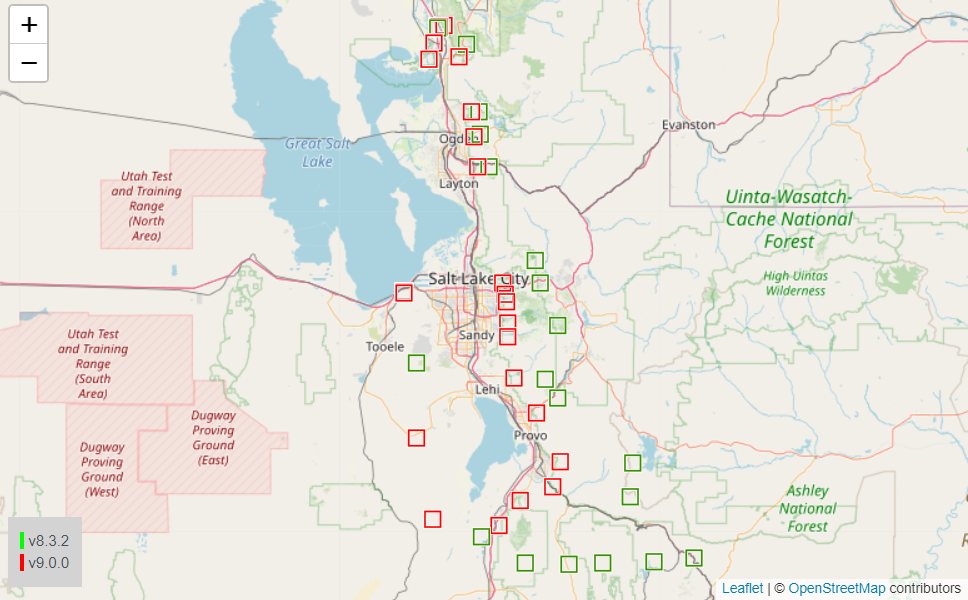
\includegraphics{v9x/v900/whats-new/_pictures/externals.png}

}

\caption{\label{fig-externals-pdf}v9 External Description.}

\end{figure}

The updated numbering scheme can be found in Figure~\ref{fig-descrip1},
Figure~\ref{fig-descrip2}, and Figure~\ref{fig-descrip3}.

\begin{figure}[H]

{\centering 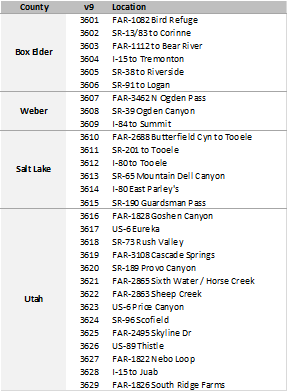
\includegraphics{v9x/v900/whats-new/_pictures/ex_descrip1.png}

}

\caption{\label{fig-descrip1}v9 External Description.}

\end{figure}

\begin{figure}[H]

{\centering 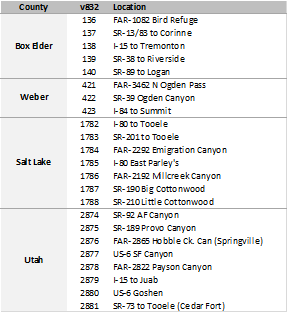
\includegraphics{v9x/v900/whats-new/_pictures/ex_descrip2.png}

}

\caption{\label{fig-descrip2}v8.3.2 External Description.}

\end{figure}

\begin{figure}[H]

{\centering 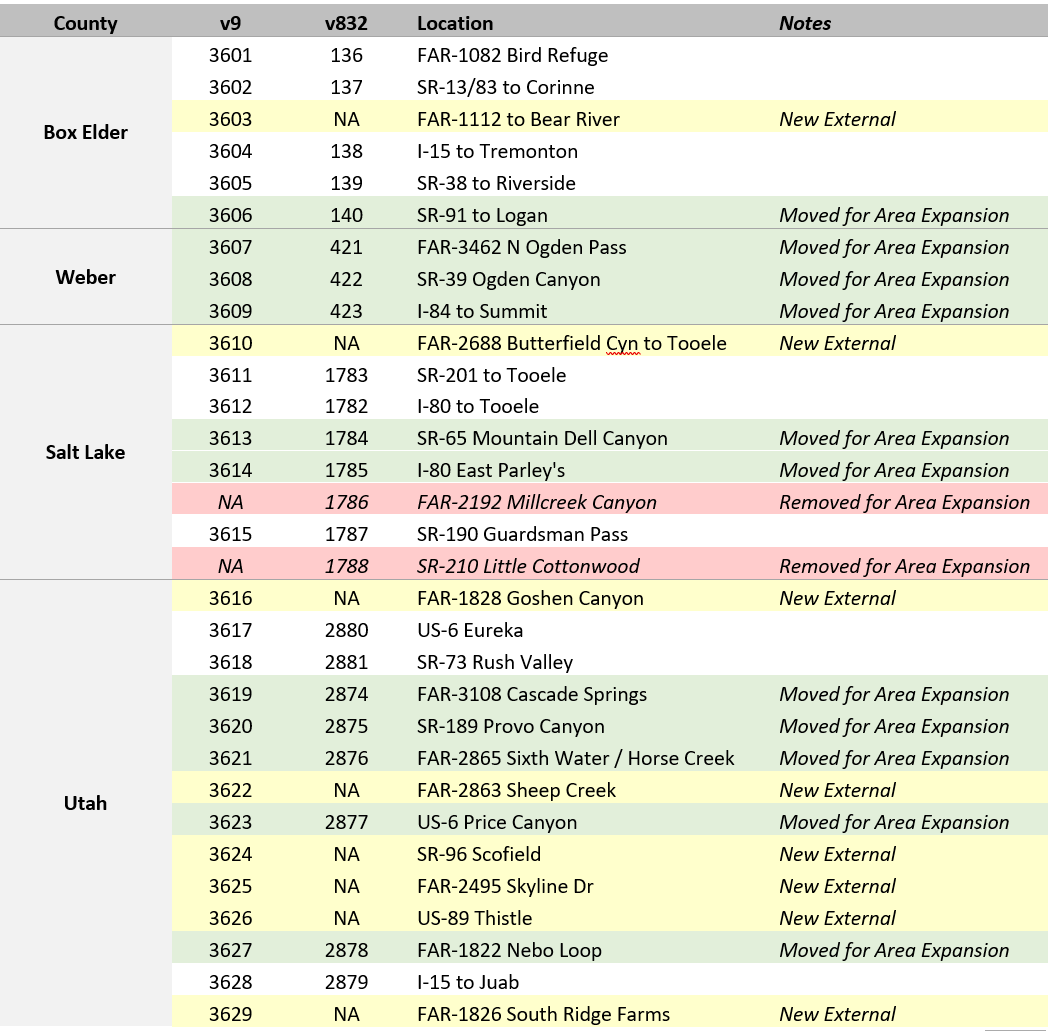
\includegraphics[width=0.5\textwidth,height=\textheight]{v9x/v900/whats-new/_pictures/ex_descrip3.png}

}

\caption{\label{fig-descrip3}v9 \& v8.3.2 External Description.}

\end{figure}

\hypertarget{segment}{%
\section{Segment}\label{segment}}

The \texttt{Master\_Segs\_withFactors\_20220915.shp} file contains the
updated segments to align with 2023 RTP network changes. Additional
segments for rail transit corridors were added in the Wasatch Front
area.

\bookmarksetup{startatroot}

\hypertarget{input-processing}{%
\chapter{Input Processing}\label{input-processing}}

Changes made to the
\texttt{2\_ModelScripts\textbackslash{}0\_InputProcessing} folder are
discussed in this section.

Global changes made to all the scripts in this folder included
modifications to the script to account for removal of the \texttt{CITY},
\texttt{COUNTY}, and \texttt{EXTERNAL} fields from the TAZ shapefile and
updates to use true shape link and node shapefiles.

\hypertarget{setup}{%
\section{Setup}\label{setup}}

The folder setup routine was integrated into the \texttt{HailMary.s}
script to run automatically. It is no longer necessary to copy empty
folders or run the \texttt{\_CreateOutputFolders.s} prior to running the
model .

\hypertarget{se-processing}{%
\section{SE Processing}\label{se-processing}}

The \texttt{1\_DemographicsAnalysis.s} script was updated to read \\
\texttt{ControlTotal\_SE\_AllCounties.csv}. Weber County contains two
sets of indexes bus on whether it is the UDOT Subarea \texttt{9057} or
the Wasatch Front Subarea \texttt{9157}.

\hypertarget{network-processing}{%
\section{Network Processing}\label{network-processing}}

A bug in the Connected-and-Autonomous Vehicle (CAV) calculation was
fixed where the column index was needed to be incremented by 1 to link
up with lookup tables.

The hard-coded turn penalty node numbers in the
\texttt{3\_TurnPenalty.s} script were updated to the new master network
node numbering.

\hypertarget{time-of-day-factors}{%
\section{Time of Day Factors}\label{time-of-day-factors}}

A new file \texttt{1\_CalculateTimeOfDayFac.s} is created during the
model that includes time of day factors for use in following scripts.

\bookmarksetup{startatroot}

\hypertarget{household-disaggregation-and-auto-ownership-1}{%
\chapter{Household Disaggregation and Auto
Ownership}\label{household-disaggregation-and-auto-ownership-1}}

The \texttt{1\_LifeCycle.s} script was modified to account for removal
of the \texttt{COUNTY} field from the TAZ shapefile and for the removal
of county-specific id variables from
\texttt{0\_GeneralParameters.block}.

\bookmarksetup{startatroot}

\hypertarget{distribution}{%
\chapter{Distribution}\label{distribution}}

Changes made to the
\texttt{2\_ModelScripts\textbackslash{}3\_Distribute} folder are
discussed in this section. The changes described in this section were
made exclusively in the \texttt{1\_Distribution.s} script.

\hypertarget{convergence}{%
\section{Convergence}\label{convergence}}

The convergence criteria was updated for trip table and link
convergences, as well as the check criteria.

\hypertarget{trip-table-convergence}{%
\subsection{Trip Table Convergence}\label{trip-table-convergence}}

For trip table convergence, the percent change threshold was reduced
from 10\% to 7.5\%. For each iteration, only cells where the trips in
the current iterations are greater than zero are considered. Cells with
trips greater than zero are counted as significant trips and form the
denominator in the percent converged calculation.

The trip matrix cell is considered converged if:

\begin{enumerate}
\def\labelenumi{\arabic{enumi}.}
\tightlist
\item
  Percent change from previous iteration is within 7.5\%, or
\item
  Trips from the current iteration are less than 1
\end{enumerate}

With the exception that the cell is not converged if the trips from the
current iteration are greater than zero and the trips from the previous
iteration equals zero.

\hypertarget{link-convergence}{%
\subsection{Link Convergence}\label{link-convergence}}

For link volume convergence, the percent change threshold was increased
from 5\% to 7.5\%. Centroid connectors are not considered when
determining convergence. For each iteration, only cells where the trips
in the current iterations are greater than zero are considered. Cells
with trips greater than zero are counted as significant trips and form
the denominator in the percent converged calculation.

The link is considered converged if:

\begin{enumerate}
\def\labelenumi{\arabic{enumi}.}
\tightlist
\item
  Percent change from previous iteration is within 7.5\%, or
\item
  Volume from current iteration equals zero and volume from previous
  iteration equals zero.
\end{enumerate}

With the exception that the link is not converged if:

\begin{enumerate}
\def\labelenumi{\arabic{enumi}.}
\tightlist
\item
  Volume from the current iteration is greater than zero and the volume
  from the previous iteration equals zero, or
\item
  Volume from the current iteration is zero and the volume from the
  previous iteration is greater than zero.
\end{enumerate}

\hypertarget{check-criteria}{%
\subsection{Check Criteria}\label{check-criteria}}

The convergence check criteria was updated. The minimum of 5 iterations
requirement was removed. The \texttt{RGAP} parameter passthrough
variable was from moved from the block file to main script just before
each assignment call. The \texttt{EV\ RGAP} parameter is set to the
\texttt{0GeneralParameters.block} value divided by 10.

\hypertarget{reports}{%
\section{Reports}\label{reports}}

The initializing and logging of trip, vehicle-miles traveled (VMT), and
vehicle-hours traveled (VHT) variables were removed from the log file.
The trip table and link convergence reports in the log file were
updated.

The following new reports were added to better track convergence:

\begin{itemize}
\tightlist
\item
  \texttt{\_Stats\ -\ Distrib\ Assign\ -\ @RID@.csv}
\item
  \texttt{\_Stats\ -\ Distrib\ Loaded\ Net\ -\ @RID@.csv}
\item
  \texttt{\_Stats\ -\ Distrib\ Trip\ Table\ -\ @RID@.csv}
\end{itemize}

\hypertarget{other}{%
\section{Other}\label{other}}

A \texttt{@unloadednetprefix@\_@n@\_convg.net} file was added to
\texttt{Temp\textbackslash{}3\_Distribute} folder. It includes following
fields (\texttt{li.1}=current iteration, \texttt{li.2}=previous
iteration):

\begin{itemize}
\tightlist
\item
  \texttt{AM\_Cur\ =\ li.1.AM\_VOL}
\item
  \texttt{MD\_Cur\ =\ li.1.MD\_VOL}
\item
  \texttt{PM\_Cur\ =\ li.1.PM\_VOL}
\item
  \texttt{EV\_Cur\ =\ li.1.EV\_VOL}
\item
  \texttt{DY\_Cur\ =\ li.1.DY\_VOL}
\item
  \texttt{AM\_Pre\ =\ li.2.AM\_VOL}
\item
  \texttt{MD\_Pre\ =\ li.2.MD\_VOL}
\item
  \texttt{PM\_Pre\ =\ li.2.PM\_VOL}
\item
  \texttt{EV\_Pre\ =\ li.2.EV\_VOL}
\item
  \texttt{DY\_Pre\ =\ li.2.DY\_VOL}
\item
  \texttt{AM\_Diff\ =\ AM\_Cur\ -\ AM\_Pre}
\item
  \texttt{MD\_Diff\ =\ MD\_Cur\ -\ MD\_Pre}
\item
  \texttt{PM\_Diff\ =\ PM\_Cur\ -\ PM\_Pre}
\item
  \texttt{EV\_Diff\ =\ EV\_Cur\ -\ EV\_Pre}
\item
  \texttt{DY\_Diff\ =\ DY\_Cur\ -\ DY\_Pre}
\item
  \texttt{AM\_PctDiff\ =\ ABS(AM\_Diff)\ /\ AM\_Pre}
\item
  \texttt{MD\_PctDiff\ =\ ABS(MD\_Diff)\ /\ MD\_Pre}
\item
  \texttt{PM\_PctDiff\ =\ ABS(PM\_Diff)\ /\ PM\_Pre}
\item
  \texttt{EV\_PctDiff\ =\ ABS(EV\_Diff)\ /\ EV\_Pre}
\item
  \texttt{DY\_PctDiff\ =\ ABS(DY\_Diff)\ /\ DY\_Pre}
\item
  \texttt{CONVLINK\ (if\ (DY\_PctDiff\textless{}=\_ConvThreshold)\ \ CONVLINK\ =\ 1)}
\end{itemize}

\bookmarksetup{startatroot}

\hypertarget{mode-choice-1}{%
\chapter{Mode Choice}\label{mode-choice-1}}

Changes made to the
\texttt{2\_ModelScripts\textbackslash{}4\_ModeChoice} folder are
discussed in this section. Updates to the mode choice portion of the
model include transit skims and district summaries.

\hypertarget{transit-skims}{%
\section{Transit Skims}\label{transit-skims}}

Modifications to the transit skim script were made to incorporate the
new bus speeds input file.

\hypertarget{district-summaries}{%
\section{District Summaries}\label{district-summaries}}

The district summary script was modified to change \texttt{COUNTY} field
references to \texttt{CO\_FIPS} for county summaries due to removal of
field from TAZ shapefile.

\bookmarksetup{startatroot}

\hypertarget{highway-assignment}{%
\chapter{Highway Assignment}\label{highway-assignment}}

The summarize loaded networks script was modified to point the geometry
input reference to the input processing output folder instead of the
highway inputs folder.

\bookmarksetup{startatroot}

\hypertarget{model-results---comparison-with-v8.3.2}{%
\chapter{Model Results - Comparison with
v8.3.2}\label{model-results---comparison-with-v8.3.2}}

This section compares the model results between v9.0 and v8.3.2 for
roadway volumes and transit.

\hypertarget{road-volume-comparisons}{%
\section{Road Volume Comparisons}\label{road-volume-comparisons}}

The comparison between daily volumes at the segment level can be found
in Figure~\ref{fig-pdf-volume-comparison} for 2019 and 2050. Decreases
in volume in v9.0 compared to v8.3.2 are shown in blue, while increases
are shown in red.

For 2019, Salt Lake and northern Davis counties display a drop in
roadway volumes, most apparent on I-15. Weber, southern Davis, and Utah
Counties show increases. Most of the changes are relatively minor, with
the largest decreases occurring on the freeways in Salt Lake County.
However, given the large daily volume for these roadways, the percent
change is relatively low.

For 2050, there are decreases in volumes on I-15 in Salt Lake and
northern Davis counties. Weber and northern Davis counties show overall
increase in roadway volumes. Utah County shows the most change with the
two Utah Lake crossings not part of the 2050 fiscally constrained
scenario. The resulting drop in volumes is evident with increases on
I-15.

The comparison of daily medium and heavy truck volumes is found in
Figure~\ref{fig-pdf-volume-truck-comparison} for 2019 and 2050. Truck
volumes decreased in the northwest portion of Salt Lake County.

\begin{figure}

\begin{minipage}[t]{0.33\linewidth}

{\centering 

\raisebox{-\height}{

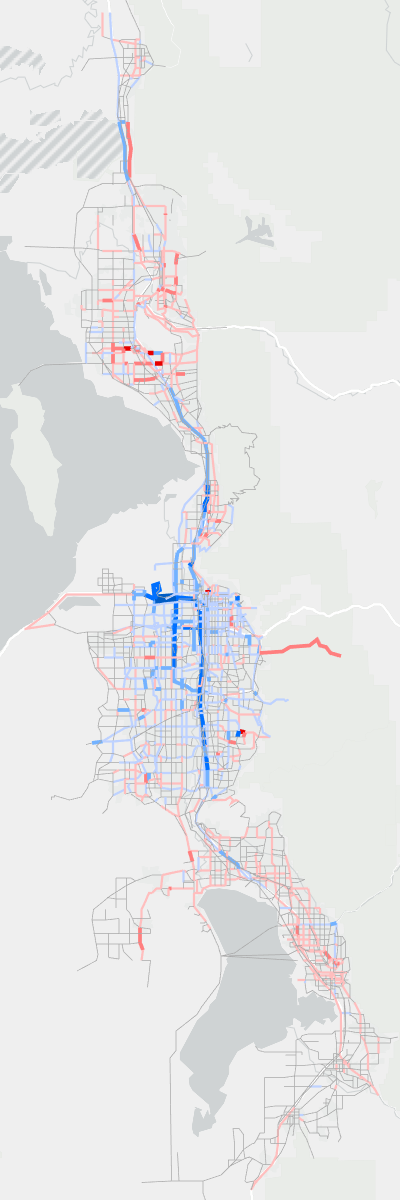
\includegraphics{v9x/v900/whats-new/data/map_pngs/vol19-cropped.png}

}

}

\subcaption{\label{fig-vol19}2019}
\end{minipage}%
%
\begin{minipage}[t]{0.33\linewidth}

{\centering 

\raisebox{-\height}{

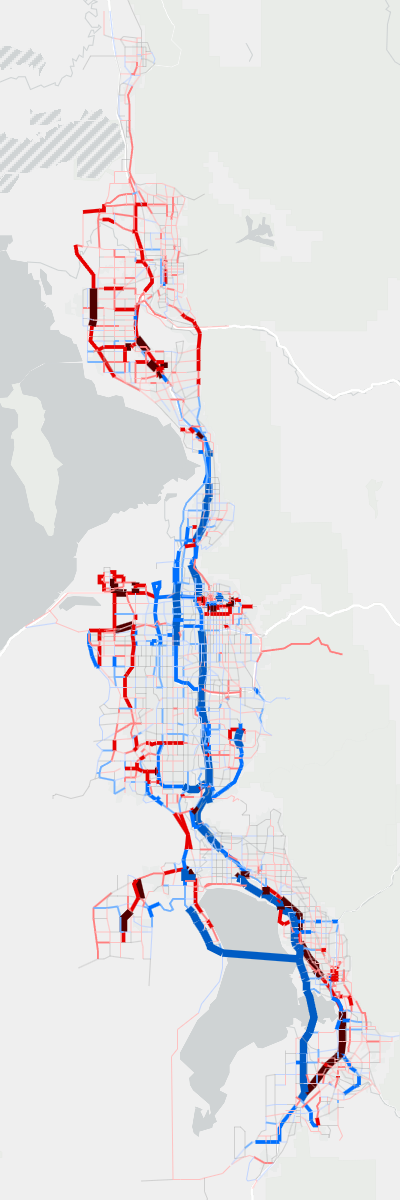
\includegraphics{v9x/v900/whats-new/data/map_pngs/vol50-cropped.png}

}

}

\subcaption{\label{fig-vol50}2050 Fiscally Constrained}
\end{minipage}%
%
\begin{minipage}[t]{0.33\linewidth}

{\centering 

\raisebox{-\height}{

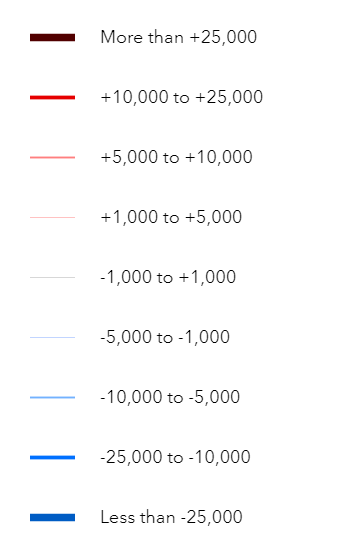
\includegraphics{v9x/v900/whats-new/data/map_pngs/vol-legend-cropped.png}

}

}

\end{minipage}%

\caption{\label{fig-pdf-volume-comparison}Model Daily Volumes Comparison
- All Vehicles (v9.0 vs v8.3.2)}

\end{figure}

\begin{figure}

\begin{minipage}[t]{0.33\linewidth}

{\centering 

\raisebox{-\height}{

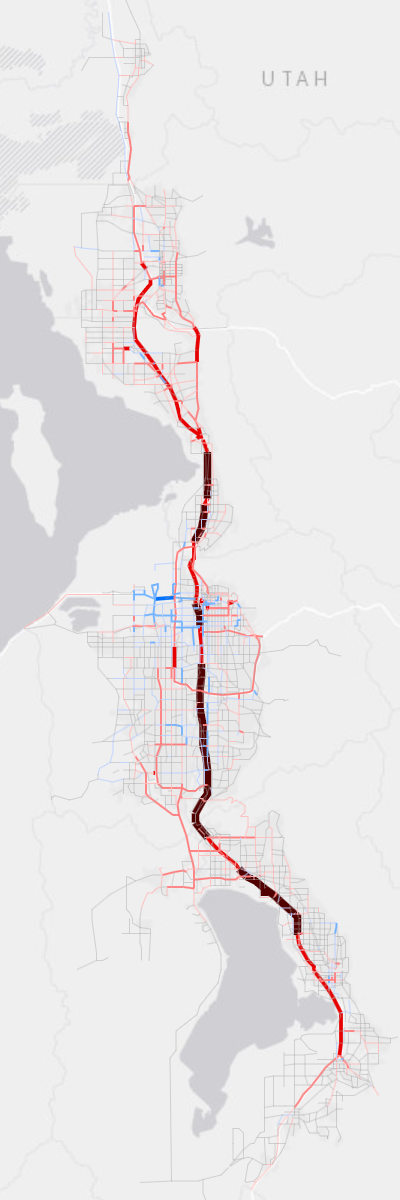
\includegraphics{v9x/v900/whats-new/data/map_pngs/vol19-truck-cropped.png}

}

}

\subcaption{\label{fig-vol19}2019}
\end{minipage}%
%
\begin{minipage}[t]{0.33\linewidth}

{\centering 

\raisebox{-\height}{

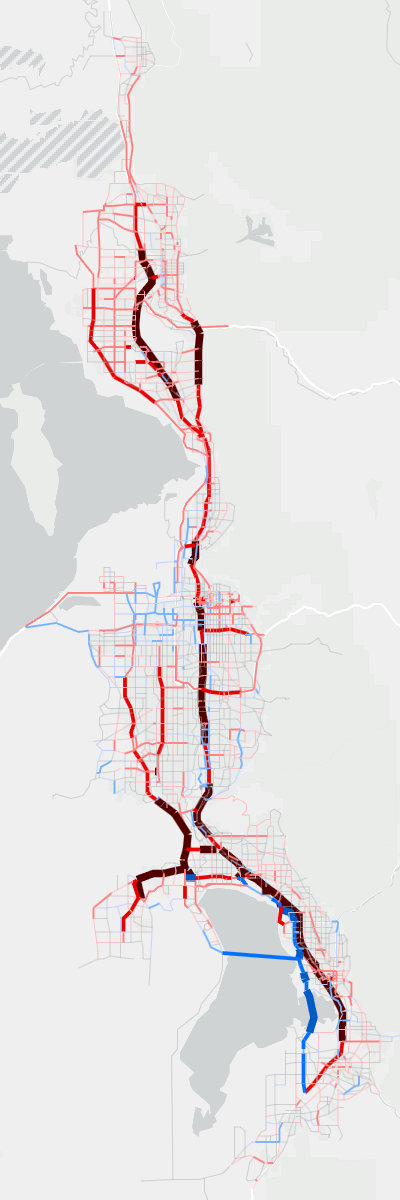
\includegraphics{v9x/v900/whats-new/data/map_pngs/vol50-truck-cropped.png}

}

}

\subcaption{\label{fig-vol50}2050 Fiscally Constrained}
\end{minipage}%
%
\begin{minipage}[t]{0.33\linewidth}

{\centering 

\raisebox{-\height}{

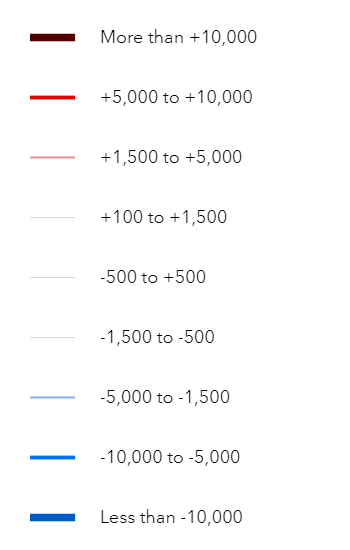
\includegraphics{v9x/v900/whats-new/data/map_pngs/vol-truck-legend-cropped.png}

}

}

\end{minipage}%

\caption{\label{fig-pdf-volume-truck-comparison}Model Daily Volumes
Comparison - Trucks (v9.0 vs v8.3.2)}

\end{figure}

\hypertarget{transit-comparisons}{%
\section{Transit Comparisons}\label{transit-comparisons}}

Transit comparisons were done with ridership, trips mode share, and
boardings mode share. Overall ridership increases significantly in v9.0,
and Core Bus ridership takes a larger share of trips and boardings than
in v8.3.2.

\hypertarget{transit-ridership}{%
\subsection{Transit Ridership}\label{transit-ridership}}

Transit ridership in v9.0 compared to v8.3.2 shows significant increase
in 2032, 2042, and 2050. See Figure~\ref{fig-pdf-hy-tr-all}. The total
ridership in 2050 for v9.0 is 327,000 daily trips compared to the v8.3.2
model that showed 258,000 daily trips, which equates to 26\% more trips.
The additional trips is largely due to the improvements in commuter rail
with increased frequency and speed together with the change in the model
sensitivity to changes in headway.

Transit ridership by modes are shown in the following set of figures.
Light-Rail Transit sees an increase through 2028 and then a large
decrease in 2032. This large decrease can be explained by the shift of
riders from Light Rail to Core Bus routes, with a large number of core
routes coming online in 2032.

\begin{figure}[H]

{\centering 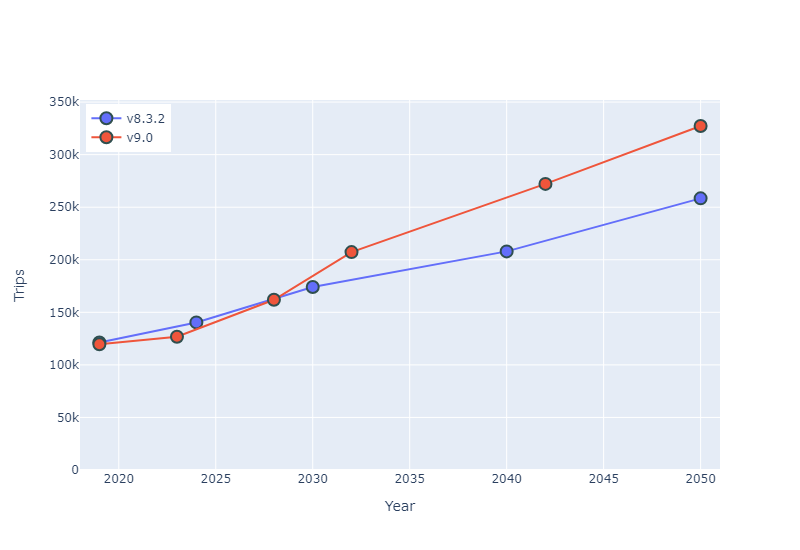
\includegraphics{v9x/v900/whats-new/_pictures/pdf-hy-tr-all.png}

}

\caption{\label{fig-pdf-hy-tr-all}Daily Transit Ridership - All Modes}

\end{figure}

\begin{figure}[H]

{\centering 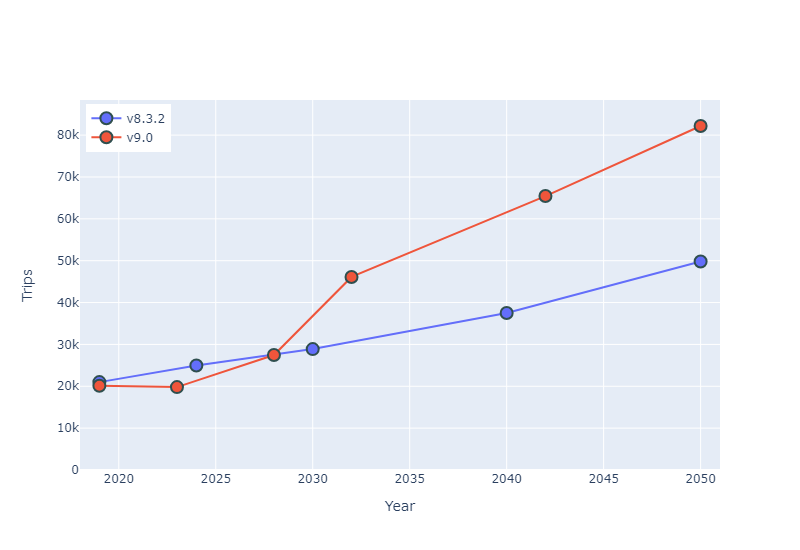
\includegraphics{v9x/v900/whats-new/_pictures/pdf-hy-tr-crt.png}

}

\caption{\label{fig-pdf-hy-tr-crt}Daily Transit Ridership -
Commuter-Rail Transit}

\end{figure}

\begin{figure}[H]

{\centering 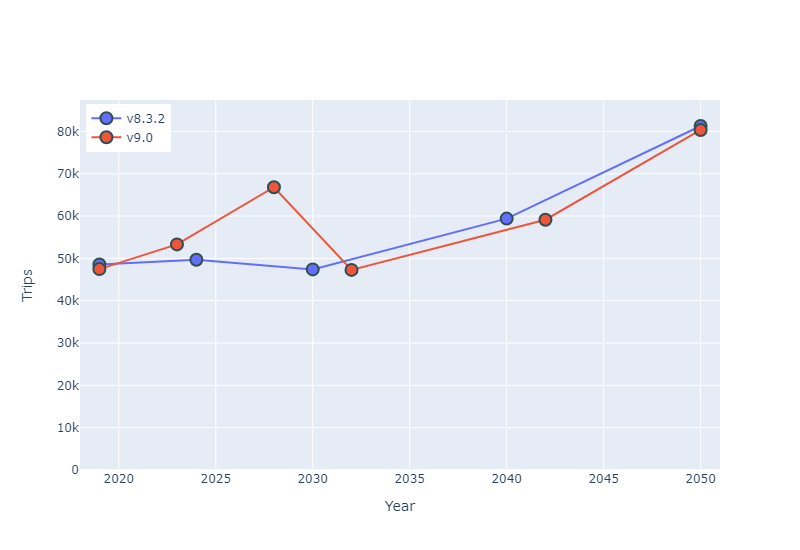
\includegraphics{v9x/v900/whats-new/_pictures/pdf-hy-tr-lrt.png}

}

\caption{\label{fig-pdf-hy-tr-lrt}Daily Transit Ridership - Light-Rail
Transit}

\end{figure}

\begin{figure}[H]

{\centering 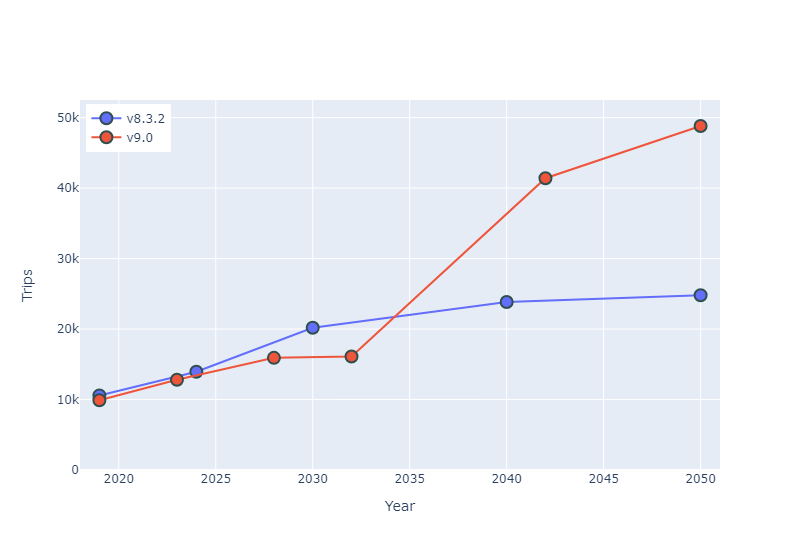
\includegraphics{v9x/v900/whats-new/_pictures/pdf-hy-tr-brt.png}

}

\caption{\label{fig-pdf-hy-tr-brt}Daily Transit Ridership - Bus Rapid
Transit}

\end{figure}

\begin{figure}[H]

{\centering 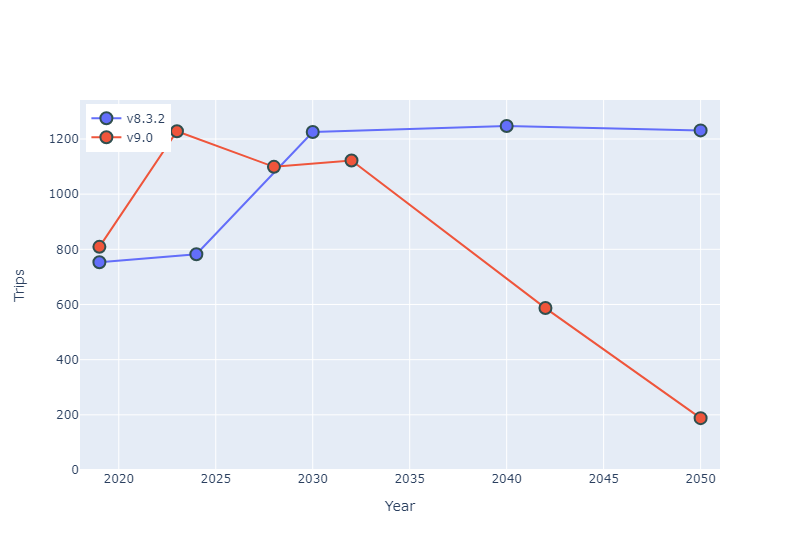
\includegraphics{v9x/v900/whats-new/_pictures/pdf-hy-tr-exp.png}

}

\caption{\label{fig-pdf-hy-tr-exp}Daily Transit Ridership - Express Bus}

\end{figure}

\begin{figure}[H]

{\centering 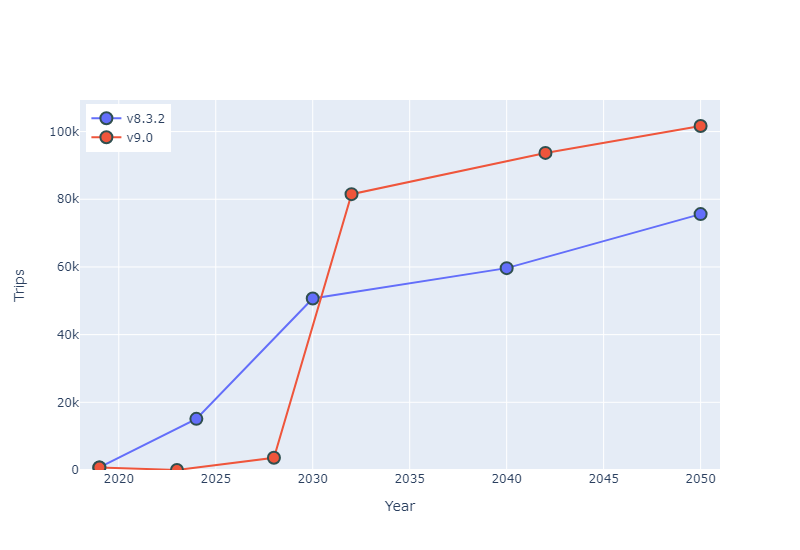
\includegraphics{v9x/v900/whats-new/_pictures/pdf-hy-tr-cor.png}

}

\caption{\label{fig-hy-tr-cor}Daily Transit Ridership - Core Bus}

\end{figure}

\begin{figure}[H]

{\centering 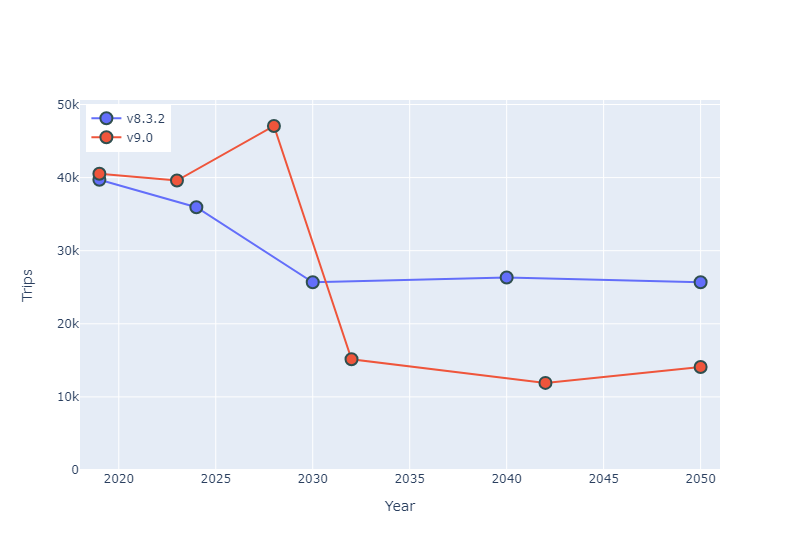
\includegraphics{v9x/v900/whats-new/_pictures/pdf-hy-tr-lcl.png}

}

\caption{\label{fig-pdf-hy-tr-lcl}Daily Transit Ridership - Local Bus}

\end{figure}

\hypertarget{transit-share}{%
\subsection{Transit Share}\label{transit-share}}

A comparison of the share of trips amongst the various modes of transit
was done for both Trips and Boardings.

The transit ridership trip shares by mode can be found in
Figure~\ref{fig-pdf-shr-tr-all-9} for v9.0 and
Figure~\ref{fig-pdf-shr-tr-all-832} for v8.3.2. The main difference in
v9.0 trip share by mode is the large increase in Core Bus trips in 2032
from almost nothing in 2028, while in v8.3.2 the increase in Core Bus
trips is spread out between 2024 and 2030. This large increase is
consistent with the transit inputs into the model with a large number of
Core Bus routes coming into production in 2032, replacing mostly local
bus service. The new Core Buy takes most of the local bus ridership it
is replacing, but also quite a lot of ridership from Light Rail Transit
(Mode 7).

Transit boardings for v9.0 are found in Figure~\ref{fig-pdf-brd-9} and
for v8.3.2 are found in Figure~\ref{fig-pdf-brd-832}. Boardings follow
the same pattern as trips, but boardings are able to differentiate
between modes better than trips that are categorized hierarchically.

\begin{figure}[H]

{\centering 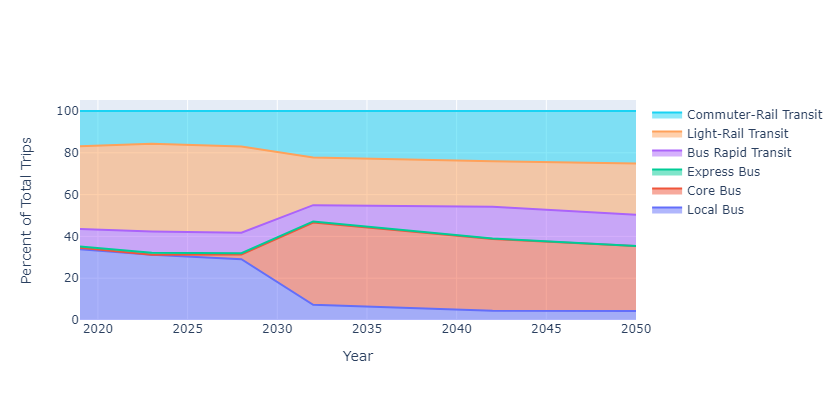
\includegraphics{v9x/v900/whats-new/_pictures/pdf-shr-tr-all-9.png}

}

\caption{\label{fig-pdf-shr-tr-all-9}Transit Trips Share by Mode - v9.0}

\end{figure}

\begin{figure}[H]

{\centering 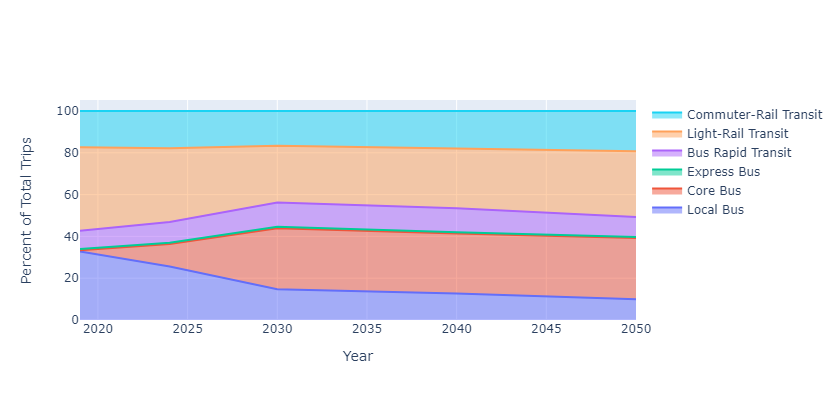
\includegraphics{v9x/v900/whats-new/_pictures/pdf-shr-tr-all-832.png}

}

\caption{\label{fig-pdf-shr-tr-all-832}Transit Trips Share by Mode -
v8.3.2}

\end{figure}

\begin{figure}[H]

{\centering 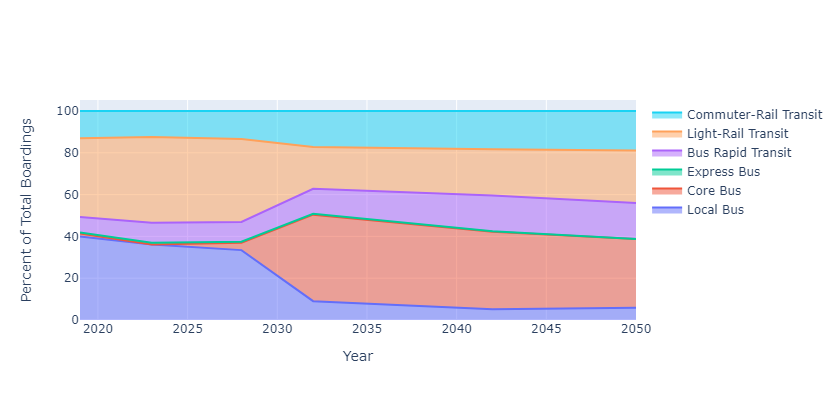
\includegraphics{v9x/v900/whats-new/_pictures/pdf-brd-9.png}

}

\caption{\label{fig-pdf-brd-9}Transit Boardings Share by Mode - v9.0}

\end{figure}

\begin{figure}[H]

{\centering 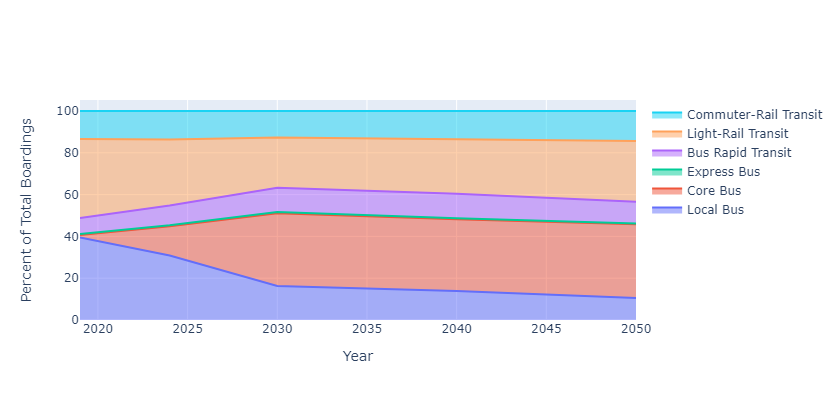
\includegraphics{v9x/v900/whats-new/_pictures/pdf-brd-832.png}

}

\caption{\label{fig-pdf-brd-832}Transit Boardings Share by Mode -
v8.3.2}

\end{figure}

\hypertarget{commuter-rail-station-boardings}{%
\subsubsection{Commuter Rail Station
Boardings}\label{commuter-rail-station-boardings}}

The comparison of base year (2019) station-level boardings for
commuter-rail transit (CRT) is found in Figure~\ref{fig-pdf-fr-brd}. CRT
boardings were found to be higher than observed for Davis County and
lower than observed for Utah County. An adjustment of 5 additional
minutes to in-vehicle-time for trips to/from Davis County and 5 fewer
minute to in-vehicle-time for Utah County was made to attempt to bring
the model more in-line with observations.

Additional investigation was conducted into why Provo and Lehi were
particularly low in the model. The findings did not turn up any obvious
errors in the transit or model network. So, the conclusion is that
further adjustments to CRT will be possible in the Mode Choice Update
project that is currently being undertaken for the next release of the
model.

\begin{figure}[H]

{\centering 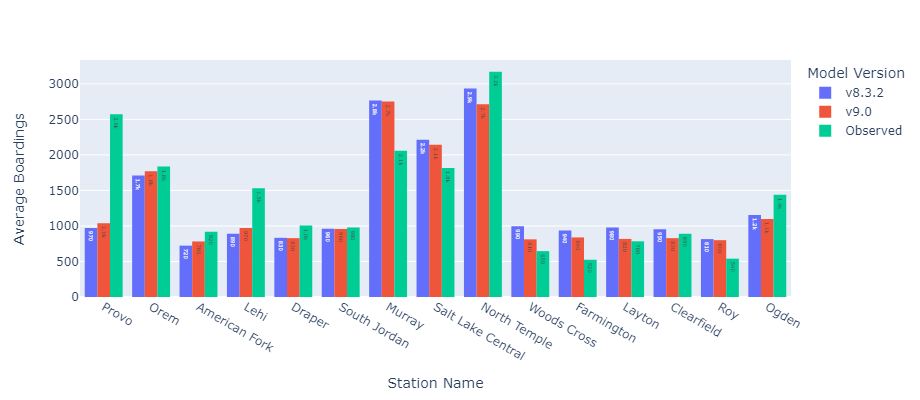
\includegraphics{v9x/v900/whats-new/_pictures/pdf-fr-brd.png}

}

\caption{\label{fig-pdf-fr-brd}2019 Daily CRT Boardings by Station -
Model vs Observed}

\end{figure}



\end{document}
